\input{./econtexRoot.tex}\providecommand{\econtex}{\econtexRoot/texmf-local/tex/latex/econtex}
\providecommand{\econtexSetup}{\econtexRoot/texmf-local/tex/latex/econtexSetup}
\providecommand{\econtexShortcuts}{\econtexRoot/texmf-local/tex/latex/econtexShortcuts}
\providecommand{\econtexBibMake}{\econtexRoot/texmf-local/tex/latex/econtexBibMake}
\providecommand{\econtexBibStyle}{\econtexRoot/texmf-local/bibtex/bst/econtex}
\providecommand{\notes}{\econtexRoot/texmf-local/tex/latex/handout}
\providecommand{\handoutSetup}{\econtexRoot/texmf-local/tex/latex/handoutSetup}
\providecommand{\handoutShortcuts}{\econtexRoot/texmf-local/tex/latex/handoutShortcuts}
\providecommand{\handoutBibMake}{\econtexRoot/texmf-local/tex/latex/handoutBibMake}
\providecommand{\handoutBibStyle}{\econtexRoot/texmf-local/bibtex/bst/handout}

  
\providecommand{\be}{\begin{equation}}
\providecommand{\ee}{\end{equation}}
\providecommand{\boldred}[1]{{\color{red}\textbf{#1}}}
\providecommand{\CEA}{\text{CEA}}
\providecommand{\Uexp}{\texttt{UExp}}
\providecommand{\showEstTime}[1]{} 

\hyphenation{non-du-ra-bles}

\newlength{\defbaselineskip}
\setlength{\defbaselineskip}{\baselineskip}
\providecommand{\setlinespacing}[1]%
           {\setlength{\baselineskip}{#1 \defbaselineskip}}
\providecommand{\lllskip}{1}

\documentclass[titlepage]{\econtex}

\usepackage{\econtexSetup}\usepackage{\econtexShortcuts}
\providecommand{\texname}{cssUSSaving}% Keyname for the bibtex entry corresponding to this paper
\usepackage{layouts,rotating,psfrag,amssymb}

\provideboolean{ifWeb} 
\setboolean{ifWeb}{false}
\ifdvi{\setboolean{ifWeb}{true}}\fi
\opt{Web}{\setboolean{ifWeb}{true}}

\ifthenelse{\boolean{ifWeb}}{\usepackage{grfext}
\PrependGraphicsExtensions*{.svg,.jpg,.JPG,.png,.PNG,.pdf,.PDF}
}{}

%\opt{JournalFormatting}{\renewcommand{\footnote}{\endnote}\RequirePackage[noheads,nolists,tablesfirst,nomarkers]{endfloat}\renewcommand{\efloatseparator}{\mbox{}}}

\opt{EndFloats}{\RequirePackage[noheads,nolists,tablesfirst,nomarkers]{endfloat}\renewcommand{\efloatseparator}{\mbox{}}}

\hypersetup{pdfauthor={Christopher Carroll <ccarroll@jhu.edu>, Jiri Slacalek <jiri.slacalek@ecb.europa.eu>, Martin Sommer <msommer@imf.org>},
            pdfsubject={Dissecting Saving Dynamics: Measuring Credit, Wealth and Precautionary Effects},
            pdfkeywords={Consumption, Saving, Wealth, Credit Availability, Uncertainty; JEL: E21, E32
            },
            pdfproducer = {LaTeX with hyperref and thumbpdf},
            pdfcreator = {ps2pdf, pdfwrite}
            }

\definecolor{Cerulean}{rgb}{0,0.48,0.652}
\DeclareMathOperator*{\argmin}{arg\,min}

\begin{document}\bibliographystyle{\econtexBibStyle}
\hfill{\tiny \texname, \today}

\begin{verbatimwrite}{\texname.title}
Dissecting Saving Dynamics: Measuring Wealth, Precautionary, and Credit Effects
\end{verbatimwrite}

% \title{Dissecting Saving Dynamics: \\ \Large \medskip Measuring Wealth, Precautionary, and Credit Effects \\ \phantom{\tiny{.}} }
\title{Dissecting Saving Dynamics: Measuring Wealth, Precautionary, and Credit Effects  }

\medskip\medskip

%\newcommand{\forceSpace}{\ifdvi {\tiny .} \fi} % For html version, kludge to force a space to be inserted
\author{
{Christopher Carroll\tiny{~}}\authNum \\ {\small JHU}
\and
{Jiri Slacalek\tiny{~}}\authNum \\ {\small ECB}
\and
{Martin Sommer\tiny{~}}\authNum \\ {\small IMF}
}

\date{January 24, 2019}

\maketitle

% \aspublished{\phantom{\tiny{.}}}

%\maketitleWithForcedDate{February 17, 2013} %\boldred{Preliminary Draft}}
% CDC: 2013-01-30: AppendixSeverance provides derivation of formulae when severance payment exists
% CDC: 2013-02-17: AppendixSeverance updated to correct minor discrepancy with code
\keywords{Consumption, Saving, Wealth, Credit, Uncertainty}
\jelclass{E21, E32}


\begin{abstract}\ifthenelse{\boolean{ifWeb}}{\Large}{}
  We argue that the U.S.\
  personal saving rate's long stability (1960s--1980s), subsequent
  steady decline (1980s--2007), and recent substantial rise
  (2008--2011) can be interpreted using a parsimonious `buffer stock'
  model of consumption in the presence of labor income uncertainty and
  credit constraints. In the model, saving depends upon the gap
  between `target' and actual wealth, with the target determined by
  credit conditions and uncertainty.  An estimated structural version
  of the model suggests that increased credit availability accounts
  for most of the long-term saving decline, while fluctuations in
  wealth and uncertainty capture the bulk of the business-cycle
  variation.
\ifthenelse{\boolean{ifWeb}}{\Large}{}
\end{abstract}

\parbox{\textwidth}{
\begin{center}
\begin{tabbing}
\texttt{Archive:~} \= \= \url{http://econ.jhu.edu/people/ccarroll/papers/cssUSSaving.pdf} \kill \\  % This line establishes the locations of the tabs, but is not printed because of the \kill directive
\texttt{~~~~Web:~} \> \> \url{http://econ.jhu.edu/people/ccarroll/papers/cssUSSaving/} \\
\texttt{~~~~PDF:~} \> \> \url{http://econ.jhu.edu/people/ccarroll/papers/cssUSSaving.pdf} \\
%\texttt{~BibTeX:~} \> \> \url{http://econ.jhu.edu/people/ccarroll/papers/cssUSSaving-Self.bib} \\
\texttt{~Slides:~} \> \> \url{http://econ.jhu.edu/people/ccarroll/papers/cssUSSaving-Slides.pdf} \\
%\texttt{Archive:~} \> \> \url{http://econ.jhu.edu/people/ccarroll/papers/cssUSSaving.zip} \\
\texttt{~~~Code:~} \> \> \href{http://econ.jhu.edu/people/ccarroll/papers/cssUSSaving/Code/Mathematica-ReadMe.txt}{\texttt{BufferStockTheory-Mathematica-Code}} \\
\texttt{~~~~~~~~~} \> \> {\it (Contains data and estimation software producing paper's results)}
\end{tabbing}
\end{center}
}

\begin{authorsinfo}
\name{Carroll: \href{mailto:ccarroll@jhu.edu}{\texttt{ccarroll@jhu.edu}}, Department of Economics, Wyman Hall 590,
Johns Hopkins University, Baltimore, MD 21218, \url{http://econ.jhu.edu/people/ccarroll/}, and National Bureau of Economic Research.}
\name{Slacalek: \href{mailto:jiri.slacalek@ecb.europa.eu}{\texttt{jiri.slacalek@ecb.europa.eu}}, European Central Bank, Frankfurt am Main, Germany, \url{http://www.slacalek.com/}. }
\name{Sommer: \href{mailto:msommer@imf.org}{\texttt{msommer@imf.org}}, International Monetary Fund, Washington, DC, \url{http://martinsommeronline.googlepages.com/}.}
\end{authorsinfo}

\thanks{We thank Andra Buca, Kerstin Holzheu, Geoffrey Keim, and Joanna S{\l}awatyniec for excellent research assistance, and John Duca, Karen Dynan, Robert Gordon, Bob Hall, Mathias Hoffmann, Charles Kramer, David Laibson, Mar\'\i a Luengo-Prado, Bartosz Ma\'ckowiak, John Muellbauer, Valerie Ramey, Ricardo Reis, David Robinson, Damiano Sandri, Jonathan Wright and seminar audiences at the Bank of England, CERGE--EI Prague, the ECB, the Goethe University Frankfurt, the 2011 NBER Summer Institute, and the 2012 San Francisco Fed conference on ``Structural and Cyclical Elements in Macroeconomics'' for insightful comments. We are grateful to Abdul Abiad, John Duca, John Muellbauer, and Anthony Murphy for sharing their datasets. The views presented in this paper are those of the authors, and should not be attributed to the International Monetary Fund, its Executive Board, or management, or to the European Central Bank.}

\titlepagefinish

\setcounter{page}{1}

\begin{figure}
\caption{Personal Saving Rate in 2007--2011 and Previous Recessions}
%\begin{center}
\label{fSRrec}
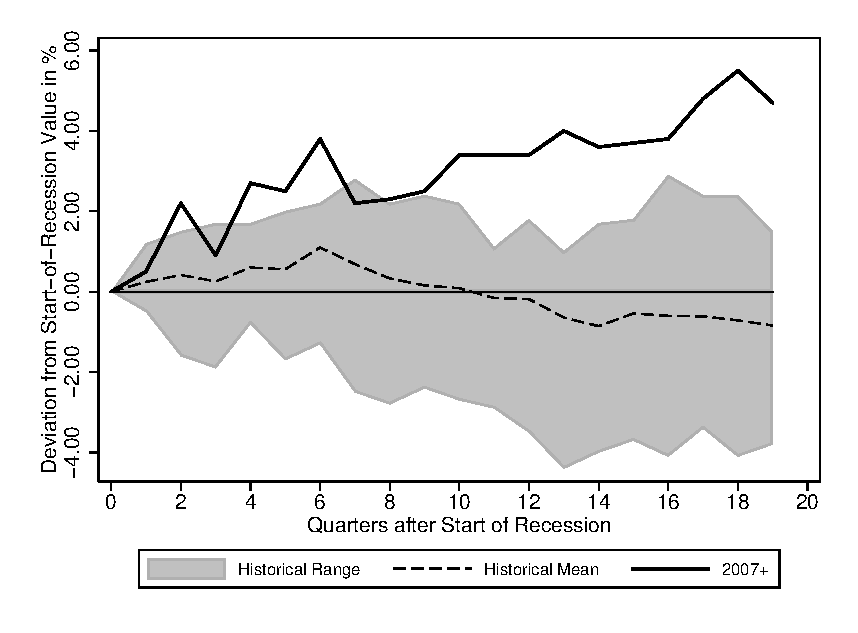
\includegraphics{\econtexRoot/Figures/saving}
%\end{center}
\footnotesize Notes: The saving rate is expressed as a percent of disposable income. The figure shows the deviation from its value at the start of recession (in percentage points). Historical Range includes all recessions after 1960q1 (when quarterly data become available).\\[-2mm]

\tiny Sources: U.S.\ Department of Commerce, Bureau of Economic Analysis.
\end{figure}

\section{Introduction}
 

The remarkable rise in personal saving during the Great Recession has sparked fresh interest in the determinants of saving decisions.  In the United States, the increase in household saving since 2007 was generally sharper than after any other postwar recession (see Figure~\ref{fSRrec}), and the personal saving rate has remained well above its pre-crisis value for the past five years.\footnote{We focus on the U.S.\ because of its central role in triggering the global economic crisis, and because of the rich existing literature studying U.S.\ data; but the U.K., Ireland, and many other countries also saw substantial increases in personal saving rates.  See~\cite{mosPSinGR} for systematic international evidence.}  While the saving rise partly reflected a decline in spending on durable goods, spending on nondurables and services was also unprecedentedly weak.\footnote{Complex issues of measurement, such as the appropriate treatment of durables, the proper role and measurement of defined benefit pension plan status, the extent to which households pierce the corporate veil, and many others, make analysis of the personal saving rate as measured by the National Income and Product Accounts a problematic enterprise.  Since there are few satisfactory solutions to any of these problems, our approach is to ignore them all, following a long tradition in (some of) the literature.  See \cite{kmitchSaving}, \cite{prSaving}, and \cite{CBOSaving} for detailed discussion of these and other measurement issues.}

\cite{carroll:brookings} invoked precautionary motives to explain the tendency of saving to increase during recessions, showing that an older modeling tradition\footnote{See \cite{davis&palumbo:wealtheffects} for an exposition, estimation, and review.}  emphasizing the role of ``wealth effects'' did not capture cyclical dynamics adequately, particularly for the first of the `postmodern'\footnote{\cite{krugmanPostmodern} seems to have coined the term `postmodern' to capture the change in the pattern of business cycle dynamics dating from the 1990--91 recession (particularly the slowness of employment to recover compared to output).  But the pattern has been noted by many other macroeconomists.} recessions in 1990--91 when wealth changed little but both saving and unemployment expectations rose markedly.

A largely separate literature has addressed another longstanding puzzle: The steady decline in the U.S.\ personal saving rate,
from over 10 percent of disposable income in the early 1980s to a mere
1 percent in the mid-2000s;\footnote{We should note here that personal saving rates tend to be one of the
most heavily revised data series in the NIPA accounts, and that substantial revisions can occur even many years after the BEA's ``first final'' estimates are made (\cite{nsSavingRevisions}, \cite{consumerGEP}); the revisions are systematically upward-biased, and often as much as 1--2 percent, so it would not be surprising if some years from now the saving decline in the 2000s appears to be smaller than in the data used here.  It seems very unlikely, however, that either the broad trends or the business-cycle frequency movements will be revised greatly; past revisions have tended to be at medium frequencies, and not at either the very low or very high frequencies that tend to provide most of our identification.}$^{,}$\footnote{
Although NIPA accounting
  conventions impart an inflation-related bias to the measurement of
  personal saving, the downward trend in saving remains obvious even
  in an inflation-adjusted measure of the saving rate.} here, a
prominent theme has been the role of financial liberalization in
making it easier for households to borrow.\footnote{See
\cite{parker_nberma_spendthrift} for a comprehensive
analysis; see \cite{admmmCredit} for comparative evidence from the U.S.,
  the U.K., and Japan emphasizing the role of credit conditions in determining saving in all three countries.} Some very recent work (\cite{glLiq}, \cite{gkLiq}, \cite{hall:slump})
has argued (though without much attempt at quantification; see however~\cite{hallQuantifying} for such an attempt) that a
sudden sharp reversal of this credit-loosening trend played a large
role in the recent saving rise.\footnote{A new paper by \cite{challe&ragot:precautionaryS}
calibrates a quantitative model with aggregate and idiosyncratic
uncertainty and time-varying precautionary saving, and documents
that the model can produce a plausible response of consumption to
aggregate shocks.
\\
\cite{alanCrossleyLow:rainyDay} simulate a model with idiosyncratic uncertainty and find that the rise of the saving rate in the recessions is driven by increase in uncertainty rather than tightening of credit.
}

This paper aims to quantify these three channels, both over the long
span of historical experience and for the period since the beginning
of the Great Recession.

To fix ideas, the paper begins by presenting (in
section~\ref{ssTractableBS}) a tractable `buffer stock' saving model
with explicit and transparent roles for each of the influences
emphasized above (the precautionary, wealth, and credit channels).
The model's key intuition is that, in the presence of income
uncertainty, optimizing households have a target wealth ratio that
depends on the usual theoretical considerations (risk aversion, time
preference, expected income growth, etc), and on two features
that have been harder to incorporate into analytical models: The degree
of labor income uncertainty and the availability of credit.  Our model
yields a tractable analytical solution that can be used to calibrate
how much saving should go up in response to an increase in
uncertainty, or a negative shock to wealth, or a tightening of
liquidity constraints.

We highlight one particularly interesting implication of the model: In response to a permanent worsening in economic circumstances (such as a permanent increase in unemployment risk), consumption initially `overshoots' its ultimate permanent adjustment.  This reflects the fact that, when the target level of wealth rises, not only is a higher level of steady-state saving needed to maintain a higher target level of wealth, an immediate {\it further} boost to saving is necessary to move from the current (inadequate) level of wealth up to the new (higher) target.  An interesting implication is that if the economy suffers from adjustment costs (as macroeconomic models strongly suggest), an optimizing government might wish to counteract the component of the consumption decline that reflects `overshooting.'  In an economy rendered non-Ricardian by liquidity constraints and/or uncertainty, this provides a potential rationale for countercyclical fiscal policy, either targeted at households or to boost components of aggregate demand other than household spending in order to offset the temporary downward overshooting of consumption.

After section~\ref{DataAndMeasurement}'s discussion of data and measurement issues, section~\ref{sReducedFormRegressions} presents a reduced-form empirical model, motivated by the theory, that attempts to measure the relative importance of each of these three effects (precautionary, wealth, and credit) for the U.S.\ personal saving rate.  An OLS analysis of the personal saving rate finds a statistically significant and economically important role for all three explanatory variables.  The model's estimated coefficients imply that the largest contributor to the decline in consumption during the Great Recession was the collapse in household wealth, with the increase in precautionary saving also making a substantial contribution; the role of measured changes in credit availability is estimated to have played a substantially smaller (though not negligible) role.

Section~\ref{sStructuralEstimation} constructs a more explicit relationship between the theoretical model and the empirical results, by making a direct identification between the model's parameters (like unemployment risk) and the corresponding empirical objects (like households' unemployment expectations constructed using the Thomson Reuters/University of Michigan's Surveys of Consumers).  We show that the structural model fits the data essentially as well as the reduced form model, but with the usual advantage of structural models that it is possible to use the estimated model to provide a disciplined investigation of quantitative theoretical issues such as whether there is an interaction between the precautionary motive and credit constraints.  (We find some evidence that there is).

\begin{comment}
Of course, \cite{keynes:generaltheory} famously argued that an
important cause of the Great Depression was a self-destructive
increase in saving that he memorably stigmatized as reflecting a
`paradox of thrift.'  While NIPA data are not available from before
the Great Depression, there seems to be little doubt that such a
saving rise did occur; but despite an insightful discussion of a
number of plausible explanations for the saving rise, Keynes did not
attempt to quantify the relative or absolute importance of those
explanations.
\end{comment}



\section{Theory: Target Wealth and Credit Conditions} \label{ssTractableBS}

\cite{ctDiscrete} (henceforth CT) provide a tractable framework for
analyzing the impact of nonfinancial uncertainty (proxied by a measure
of unemployment risk), on optimal household saving.  \cite{cjSOE} show
that the lessons from the individual's problem, solved below, carry
over with little modification to the characterization of the behavior
of aggregate variables in a small open economy.  A satisfactory
closed-economy general equilibrium analysis remains elusive (though
see \cite{challe&ragot:precautionaryS} for a valiant effort.)  Such an
analysis would be useful because a crucial question is the extent to
which each of the influences we measure is an ``impulse'' versus the
extent to which it is a ``propagation mechanism'' or a consequence of
deeper unmeasured forces.  (In the Great Recession, the collapse in
consumer confidence seems to have preceded the credit tightening; the
wealth decline began before either of the other two variables moved,
but its sharpest contractions came after both other variables had
deteriorated sharply).  In the absence of a satisfactory framework
that identifies answers to these questions, we propose that our
simple structural model at least provides a framework for organizing and
thinking about the issues.

The consumer maximizes the discounted sum of utility from an intertemporally separable CRRA utility function $\util(\bullet)=\bullet^{1-\CRRA}/(1-\CRRA)$ subject to the dynamic budget constraint:
$$
m_{t+1}=(m_t-c_t)\Rfree+\ell_{t+1}\Wage_{t+1}\xi_{t+1},
$$
where next period's market resources $m_{t+1}$ are the sum of
current market resources net of consumption $c_t$, augmented by the
(constant) interest factor $\Rfree=1+\rfree$, and with the addition of
labor income. The level of labor income is determined by the
individual's productivity $\ell$ (lower case letters designate
individual-level variables), the (upper-case) aggregate wage $\Wage_{t+1}$ (per
unit of productivity) and a zero--one indicator of the consumer's
employment status $\xi$.

The assumption that makes the model tractable is that unemployment risk takes a particularly stark form: Employed consumers face a constant probability $\mho$ of becoming unemployed, and, once unemployed, the consumer can never become employed again.\footnote{Of course, if a starting population of such consumers were not refreshed by an inflow of new employed consumers, the population unemployment rate would asymptote to 100 percent.  This problem can easily be addressed by introducing explicit demographics
  (which do not affect the optimization problem of the employed): Each
  period new employed consumers are born and a fraction of existing
  households dies, as in \cite{cjSOE}.  Because
  demographic effects are very gradual, the implications of the more
  complicated model are well captured by the simpler model presented
  here that ignores demographics and the behavior of the unemployed
  population.} Under these assumptions, CT derive a formula for the steady-state target $\check{\mRat}$ that depends on unemployment risk $\mho$, the
interest rate $\rfree$, the growth rate of wages $\Delta \Wage$,
relative risk aversion $\CRRA$, and the discount factor $\Discount$:%
\footnote{  Specifically, the steady-state target wealth can be approximated as
$$
\check{\mRat}=1+\frac{1}{\pat_r(\hat{p}_\gamma/\mho)-\pat_\gamma},
$$
where $\pat_r=\log\big((\Rfree\Discount)^{1/\CRRA}\big)\big/\Rfree$,
$\pat_\gamma=\log\big((\Rfree\Discount)^{1/\CRRA}\big)\big/\Gamma$,
$\hat{\pat}_\gamma=\pat_\gamma(1+\pat_\gamma\omega/\mho)$, $\Gamma=(1+\Delta
\Wage)/(1-\mho)$ and $\omega=(\CRRA-1)/2$.  } \be
\check{\mRat}=f(\mathop{\mho}_{(+)},\mathop{\rfree}_{(+)},\mathop{\Delta
  \Wage}_{(-)},\mathop{\CRRA}_{(+)},\mathop{\Discount}_{(+)}). \label{mTargetNonlin}
\ee Target $\mRat$ increases with unemployment risk, because in
response to higher uncertainty, consumers choose to build up a larger
precautionary buffer of wealth to protect their spending.  (The increase in $\mho$ is a pure increase in risk (a mean-preserving spread in human wealth) because
  productivity is assumed to grow by the factor $1/(1-\mho)$ each
  period, $\ell_{t+1}=\ell_t/(1-\mho)$ (see \cite{ctDiscrete}, p.\ 6)).
  A higher interest rate increases the rewards to holding wealth and thus increases the amount held. Faster income growth translates into a lower wealth target because households who anticipate higher future income consume more now in anticipation of their future prosperity (the `human wealth effect'). Finally, risk aversion and the discount factor have effects on target wealth that are qualitatively similar to the effects of uncertainty and the interest rate, respectively. While the unemployment risk in \cite{ctDiscrete} is of a simple form, the key mechanisms at work are the same as those in more sophisticated setups with a realistic specification of uninsurable risks (building on the work of \cite{bewleyPIH}, \cite{skinner_jme88}, \cite{zeldes_qje89}, \cite{deaton_ecta91}, \cite{carroll:brookings}, \cite{carroll_bufferStockSaving_qje97} and many others).

\begin{comment}
  In our empirical framework, we do not intend to identify the
  slowly-moving deep parameters such as risk aversion or the discount
  rate. Instead, we aim to estimate the dynamics of the target wealth
  with respect to risk, interest rates, and expected income growth:
  \be \check{\mRat}_t=m_0+\delta_\sigma\sigma^{2*}_{t-1}+\delta_r
  \check{\rfree}_{t-1}+\delta_y \Delta
  \PGro_{t-1}+\eta^m_t,\label{mStar} \ee where $\sigma^{2*}$ denotes
  uncertainty, $\check{\rfree}$ is the ex ante real interest rate and
  $\Delta \PGro$ denotes expected income growth. All four starred
  variables are assumed to be unobserved---target wealth is a
  theoretical construct, while the available measure of uncertainty,
  ex ante real interest rates and expected income do not perfectly
  match their (starred) theoretical counterparts.%
  \footnote{    To keep the estimation tractable, we impose a linearity of the
    model and normality of disturbances. While neither holds in
    reality, our estimation approach (which also allows for
    measurement error) yields plausible results and seems to capture
    the key properties of the data well. Ideally, we would like to
    take the estimation one step further by solving, simulating and
    estimating a realistic non-linear model of consumption choice
    under easing credit constraints and uncertainty about the relevant
    variables (including income growth, interest rates and asset
    prices). However, given the current state of knowledge, this is a
    daunting task, well beyond the scope of this paper.  }
\end{comment}

Figure~\ref{fig:PhaseDiag} shows the phase diagram for the CT model.
The consumption function is indicated by the thick solid locus, which is the
saddle path that leads to the steady state at which the ratios of
both consumption and market resources to income ($c$ and $m$) are constant.\footnote{For a detailed
intuitive exposition of the model, see \\
\url{http://econ.jhu.edu/people/ccarroll/public/lecturenotes/consumption/tractablebufferstock/}.}

\begin{figure}
\caption{Consumption Function (Stable Arm of Phase Diagram)}\label{fig:PhaseDiag}
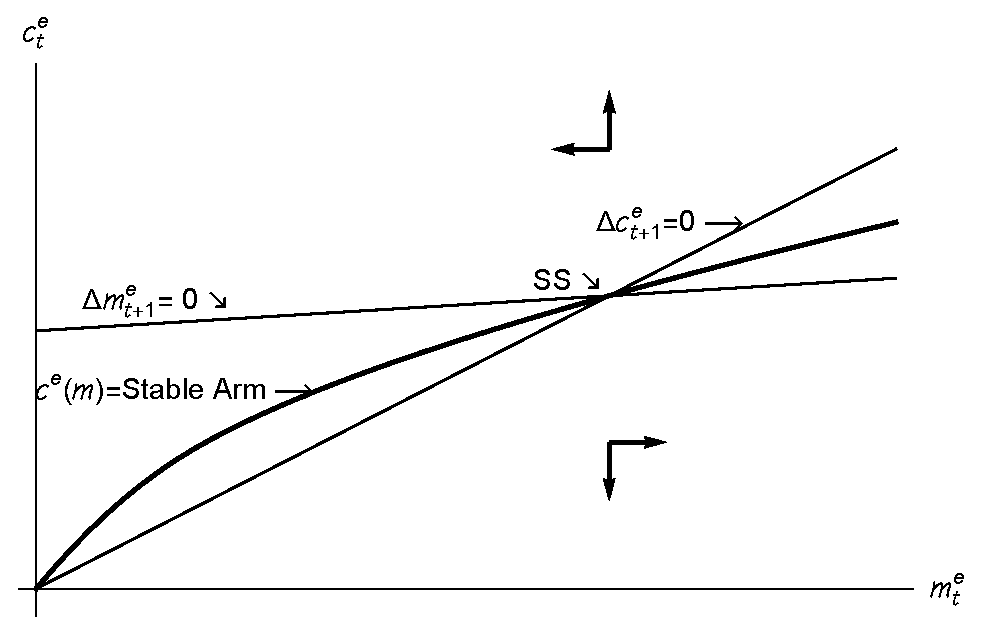
\includegraphics{\econtexRoot/Figures/TractableBufferStockPhaseDiag}
\tiny Source: Calculations by the authors using the CT  model; code generating figure is in online archive
\end{figure}

This consumption function can be used directly to analyze the consequences of an exogenous shock
to wealth of the kind contemplated in the old ``wealth effects'' literature, or in the AEA Presidential Address of \cite{hall:slump}.\footnote{Like that literature,
we take the wealth shock to be exogenous.  It is clear from the prior
literature starting with \cite{merton:restat} and \cite{samuelson:portfolio} that not much would change if a risky return were incorporated and the wealth shock were interpreted as a particularly bad realization
of the stochastic return on assets.  The much more difficult problem of constructing a plausible general equilibrium theory
of endogenous asset pricing that could justify the observed wealth shocks has not yet been satisfactorily solved, which is why we follow~\cite{hall:slump} in treating wealth shocks at the beginning of the Great Recession as exogenous.}  The consequences of a pure shock to wealth are depicted in figure~\ref{fig:WealthShock} and are straightforward: Consumption declines upon impact, to a level below the value that would leave $\mE$ constant (the leftmost red dot); because consumption is below income, $\mE$ (and thus $\cE$) rises over time back toward the original target (the sequence of dots).

\begin{figure}
%\begin{center}
\caption{A Wealth Shock}\label{fig:WealthShock}
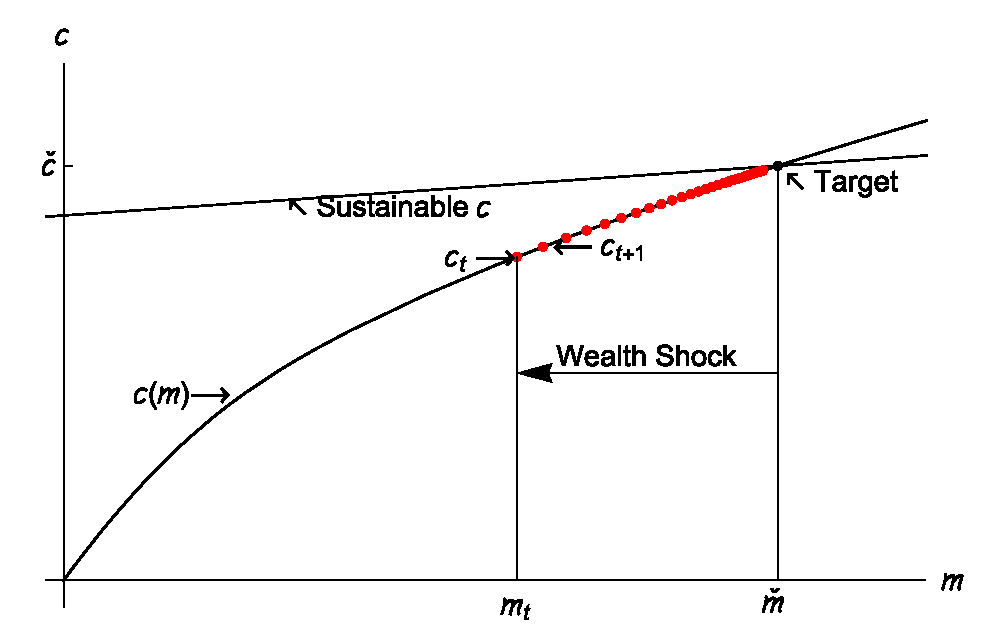
\includegraphics{\econtexRoot/Figures/WealthShock}
\tiny Source: Calculations by the authors using the CT  model; code generating figure is in online archive
%\end{center}
\end{figure}

CT's model deliberately omitted explicit liquidity constraints in order to highlight the point that uncertainty induces concavity of the consumption function (that is, a higher marginal propensity to consume for people with low levels of wealth) even in the absence of constraints (for a general proof of this proposition, see \cite{carroll&kimball:concavity}).  Indeed, because the employed consumer is always at risk of a transition into the unemployed state where income will be zero, the `natural borrowing constraint' in this model prevents the consumer from ever choosing to go into debt, because an indebted unemployed consumer with zero income might be forced to consume zero or a negative amount (incurring negative infinity utility) in order to satisfy the budget constraint.

We make only one modification to the CT model for the purpose at hand: We introduce an `unemployment insurance' system that guarantees a positive level of income for unemployed households.  In the presence of such insurance, households with low levels of market resources will be willing to borrow because they will not starve even if they become unemployed.  This change induces a leftward shift in the consumption function by an amount corresponding to the present discounted value of the unemployment benefit.  The consumer will limit his indebtedness, however, to an amount small enough to guarantee that consumption will remain strictly positive even when unemployed (this requirement defines the `natural borrowing constraint' in this model).

We could easily add a tighter `artificial' liquidity constraint, imposed exogenously by the financial system, that would prevent the consumer from borrowing as much as the natural borrowing constraint permits.  But \cite{carroll:atheoryjep} shows that the effects of tightening an artificial constraint are qualitatively and quantitatively similar to the effects of tightening the natural borrowing constraint; while we do not doubt that artificial borrowing constraints exist and are important, we do not incorporate them into our framework since we can capture their consequences by manipulating the natural borrowing constraint that is already an essential element of the model.  Indeed, using this strategy, our empirical estimates below will interpret the process of financial liberalization which began in the U.S.\ in the early 1980s and arguably continued until the eve of the Great Recession as the major explanation for the long downtrend in the saving rate.

Figure~\ref{fig:PhaseDiagramDebtLimRise} shows that the model reproduces the standard result from the existing literature (see, e.g., \cite{carroll:atheoryjep}, \cite{mue07}, \cite{glLiq}, \cite{hall:slump}): Relaxation of the borrowing constraint (from an initial position of 0.\ in which no borrowing occurs, to a new value in which the natural borrowing limit is $\underline{h}$ implying minimum net worth of $-\underline{h}$) leads to an immediate increase in consumption for a given level of resources.  But over time, the higher spending causes the consumer's level of wealth to decline, forcing a corresponding gradual decline in consumption until wealth eventually settles at its new, lower target level.  (For vivid illustration, parameter values for this figure were chosen such that
the new target level of wealth is negative; that is, the consumer would be in debt, in equilibrium).

\begin{figure}
%\begin{center}
\caption{Relaxation of a Natural Borrowing Constraint from 0 to $\underline{h}$}
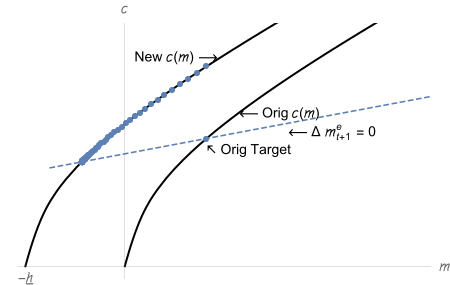
\includegraphics{\econtexRoot/Figures/PhaseDiagramDebtLimRisePlot}
\label{fig:PhaseDiagramDebtLimRise}
\tiny Source: Calculations by the authors using the CT  model; code generating figure is in the paper's online archive
%\end{center}
\end{figure}

Rather than presenting another phase diagram analysis, we
illustrate our next experiment by showing the dynamics of the
saving rate rather than the level of consumption over time.  (Since
both saving and consumption are strictly monotonic functions of $\mE$,
there is a mathematical equivalence between the two ways of presenting
the results).

% Figure depicts this relationship, illustrating the usual conclusion that saving declines with resources because the intensity of the precautionary motive lessens as wealth rises.
Figure~\ref{fig:savRateAfterMhoRisePlot} shows the consequences of a
permanent increase in unemployment risk $\urate$: An immediate jump in
the saving rate, followed by a gradual decline toward a new
equilibrium rate that is higher than the original one.


\begin{figure}
%\begin{center}
\caption{Dynamics of the Saving Rate after an Increase in Unemployment Risk}
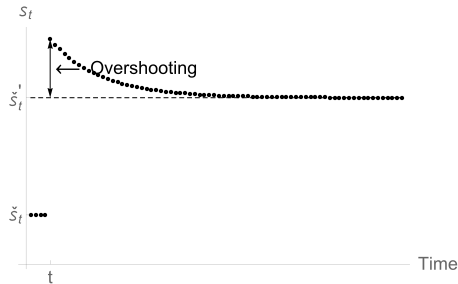
\includegraphics{\econtexRoot/Figures/savRateAfterMhoRisePlot}
\label{fig:savRateAfterMhoRisePlot}
\tiny Source: Calculations by the authors using the CT model; code generating figure is in the paper's online archive
%\end{center}
\end{figure}

Qualitatively, the effects of an increase in risk are essentially the opposite
of a credit loosening: In response to a human-wealth-preserving spread in unemployment risk, the level of
consumption falls sharply as consumers begin the process of
accumulation toward a higher target wealth ratio.\footnote{The model
  is specified in such a way that an increase in the parameter
  $\urate$ that we are calling the `unemployment risk' here actually
  induces an offsetting increase in the expected mean level of income
  (an increase in $\urate$ is a mean-preserving spread in the relevant
  sense); the spending of a consumer with certainty-equivalent
  preferences therefore would not change in response to a change in
  $\urate$, so we can attribute all of the increase in the saving rate
  depicted in the figure to the precautionary motive.}  The figure illustrates the `overshooting' proposition mentioned in the introduction: All of the initial increase in saving reflects a drop in consumption (by construction, the mean-preserving spread in unemployment risk leaves current income unchanged), and consumption recovers only gradually toward its ultimately higher target.  For a long time, the saving rate remains above either its pre-shock level or its new target.


Economists' instinct (developed in complete-markets and
perfect-foresight models) is that privately optimal behavior also
usually has a plausible claim to reflect a socially efficient
outcome.  This is emphatically {\it not} the case for movements in
precautionary saving against idiosyncratic risk in models with imperfect capital markets.  It has
long been known that such precautionary saving generates socially `excessive'
saving (see, e.g., \cite{aiyagari:opttax}).  So the presumption from
economic theory is that the increase in the precautionary motive
following an increase in uninsurable risk is socially inefficient.
The inefficiency would be even greater if we were to add to our model
a production sector like the one that has become standard in DSGE
models in which there are costs of adjustment to the amount of
aggregate investment (e.g., \cite{cee:habits}).

While the implications for optimal fiscal policy are beyond the scope
of our analysis, it is clear that a number of policies could either
mitigate the consumption decline (e.g., an increase in social
insurance) or replace the corresponding deficiency in aggregate demand
(e.g., by an increase in government spending).  We leave further
exploration of these ideas to later work, or other authors.

\begin{comment}
\begin{figure}
%\begin{center}
\caption{Increase in Unemployment Risk}\label{fig:cBeforeAndAfteruRise}
\includegraphics{\econtexRoot/Figures/cBeforeAndAfteruRise}
%\end{center}
\end{figure}
\end{comment}

One objection to the model might be that its extreme assumption about
the nature of unemployment risk (once unemployed, the consumer can
never become reemployed) calls into question its practical usefulness
except as a convenient stylized treatment of the logic of
precautionary saving.  Our view is that such a criticism would be
misplaced, for several reasons.  First, when unemployment risk is set
to zero, the model collapses to the standard Ramsey model that has
been a workhorse for much of macroeconomic analysis for the past 40
years (see~\cite{ctDiscrete} for details).  It seems perverse to
criticize the model for moving at least a step in the direction of
realism by introducing a precautionary motive into that framework.  We
have more sympathy with the view that the model's failure to
incorporate heterogeneity across types of consumers (e.g., borrowers
versus savers) misses something important (for evidence,
see~\cite{dynan_debtOverhang}, \cite{mrsBalance}, and papers cited
therein).  But this paper's authors have been active participants in
the literature that builds far more realistic models of precautionary
saving, and our considered judgment is that in the present context the
virtues of transparency and simplicity outweigh the cost in realism;
and given the model's success in matching empirical saving dynamics,
it is difficult to see how explicit incorporation of heterogeneity
could improve its fit very much quantitatively.  Models are metaphors,
not high-definition photographs, and if a certain flexibility of
interpretation is granted to use a simple model that has most of the
right parts, more progress can sometimes be made than by building a
state-of-the-art Titanic.

In sum, the model emphasizes three factors that affect saving and that might vary substantially over time.  First, because the precautionary motive diminishes as wealth rises, the saving rate is a declining function of market resources $m_{t}$.  Second, since an expansion in the availability of credit reduces the target level of wealth, looser credit conditions (designated $\CEA_t$, for reasons articulated below) lead to lower saving.  Finally, higher unemployment risk $\mho_t$ results in greater saving for precautionary reasons.

The framework thus suggests that if proxies for these variables can be
found, a reduced-form regression for the saving rate $s_t$
\begin{equation}
s_t = \gamma_0+\gamma_m m_t+
\gamma_{\CEA} \CEA_t+ \gamma_\mho \mho_t + \gamma' X_t +
\varepsilon_t \label{eqSavingReg}
\end{equation}
should satisfy the following conditions:
\be \gamma_m<0,\qquad \gamma_{\CEA}<0,\qquad \gamma_\mho>0, \ee where $\CEA_t$ denotes the ``Credit Easing
Accumulated'' index, a measure of credit supply (described in detail below), and the vector $X_t$
collects other drivers of saving that are outside the scope of the
model, such as demographics, corporate and government saving, etc.  We estimate regressions of the form
\eqref{eqSavingReg} in section~\ref{sReducedFormRegressions} below.

To economists steeped in the wisdom of Irving \cite{fisher:interestTheory}, according to whom the consumption path is determined by lifetime resources independently of the income path (`Fisherian separation holds'), equation~\eqref{eqSavingReg} may seem like a throwback to the bad old days of nonstructural Keynesian estimation of the kind that fell into disrepute after spectacular failures in the 1970s.  Below, however, we will show that, at least under our assumptions, a reduced form estimation of such an equation can in principle yield estimates of ``structural'' parameters like the time preference rate.  (An important part of the reason this exercise is not implausible is that, with the exception of a few easily identified episodes, the time path of personal income is not very far from a random walk with drift, justifying the identification of actual aggregate personal income with `permanent income' in a Friedmanian sense).\footnote{More precisely, an empirical decomposition of NIPA personal disposable income into permanent and transitory components (in which income consists of unobserved random walk with drift and white noise) assigns almost all variation in (measured) income to its permanent component, so that a ratio to actual income will coincide almost perfectly with a ratio to estimated `permanent' income. This is not surprising because, as is well-known (and also documented in Appendix~2), it is difficult to reject the proposition that almost all shocks to the level of aggregate income are permanent; autocorrelation functions and partial autocorrelation functions indicate that log-level of disposable income is close to a random walk; see our further discussion in Appendix~2.}

\section{Data and Measurement Issues} \label{DataAndMeasurement}

Before presenting estimation results we introduce our dataset.  Because our empirical measure of credit conditions begins in 1966q2, our analysis begins at that date and extends (at the present writing) through 2011q1.\footnote{Most time series were downloaded from Haver
  Analytics, and were originally compiled by the Bureau of Economic
  Analysis, the Bureau of Labor Statistics or the Federal Reserve.}$^{,}$\footnote{We are reluctant to use more recent data because personal saving rate statistics are subject to particularly large revisions until the data have been subjected to at least one annual revision (\cite{consumerGEP}; \cite{nsSavingRevisions}).} The saving rate is from the BEA's National Income and Product Accounts and is expressed as a percentage of disposable income.%
\footnote{  As a robustness check, we have also re-estimated our models with
  alternative measures of saving: Gross household saving as a fraction of disposable income, gross and net private saving as a fraction of GDP, inflation-adjusted personal saving rate and two measures of saving from the Flow of Funds (with/without consumer durables). The inflation-adjusted saving rate deducts from saving the erosion in the value of money-denominated assets due to inflation. The Flow of Funds (FoF) calculates saving as the sum of the net acquisition of financial assets and
  tangible assets minus the net increase in liabilities. Because this
  FoF-based measure is substantially more volatile, the fit of the
  model is worse than for the NIPA-based PSR. However, the main
  messages of the paper remain unchanged.  }$^{,}$\footnote{Many reasonable objections
can be made to this, or any other, specific measure of the personal saving rate, including
the treatment of durable goods, the treatment of capital gains and losses, and so on.  While
some defense of the NIPA measure could be made in response to many of these challenges, such
defenses would take us too far afield, and we refer the reader to the extensive discussions
of these measurement issues that date at least back to \cite{friedmanATheory}.}


\begin{figure}
\caption{Net Worth--Disposable Income Ratio}
%\begin{center}
\label{fwyRat}
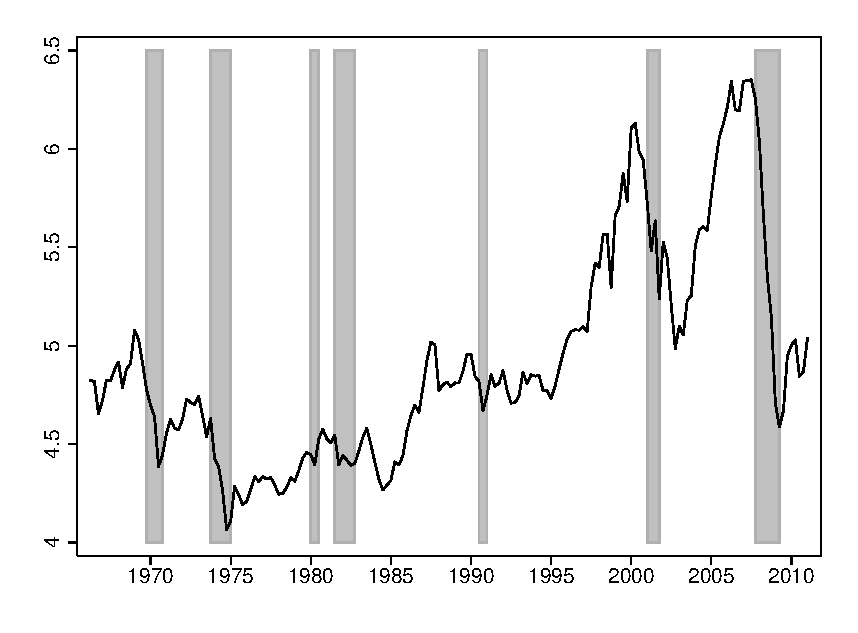
\includegraphics{\econtexRoot/Figures/fwyRat}
%\end{center}
\footnotesize
Notes: Shading---NBER recessions.\\[0mm]
\tiny Sources: Federal Reserve, Flow of Funds Accounts of the United States, \url{http://www.federalreserve.gov/releases/z1/}.
\end{figure}

Market resources $m_t$ are measured as 1 plus the ratio of household net worth to disposable income, in line with the model (Figure~\ref{fwyRat}).\footnote{This variable is lagged by one quarter to account for the fact that data on net worth are reported as the end-of-period values.}  Our measure of credit supply conditions, which we call the Credit Easing Accumulated index ($\CEA$, see Figure~\ref{fCEA}), is constructed in the spirit of \cite{mue07} and \cite{ducaEtAl10_creditArch} using the question on consumer installment loans from the Federal Reserve's Senior Loan Officer Opinion Survey (SLOOS) on Bank Lending Practices (see also \cite{fernandezMuellbauer06} and \cite{hall:slump}).  The question asks about banks' willingness to make consumer installment loans now as opposed to three months ago (we use this index because it is available since 1966; other measures of credit availability, such as for mortgage lending, move closely with the index on consumer installment loans over the sample period when both are available). To calculate a proxy for the \emph{level} of credit conditions, the scores from the survey were accumulated, weighting the responses by the debt--income ratio to account for the increasing trend in that variable.%
\footnote{  As in \cite{mue07}, we use the question on consumer installment
  loans rather than mortgages because the latter is only available
  starting in 1990q2 and the question changed in 2007q2.
  Our CEA index differs from \cite{mue07}'s Credit Conditions Index in that Muellbauer accumulates raw answers, not weighting them by the debt--income ratio.
}
  (The index is normalized between 0 and 1 to make the interpretation of regression coefficients straightforward.)

\begin{figure}
\caption{The Credit Easing Accumulated (CEA) Index}
%\begin{center}
\label{fCEA}
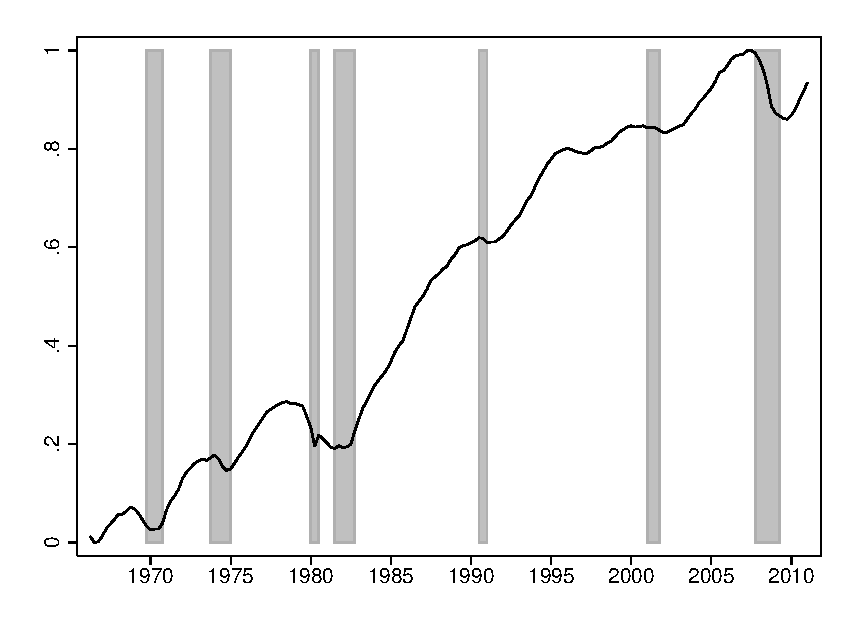
\includegraphics{\econtexRoot/Figures/fCEA}
%\end{center}
\footnotesize
Notes: Shading---NBER recessions.\\[0mm]
\tiny Sources: Federal Reserve, accumulated scores from the question on change in the banks' willingness to provide consumer installment loans from the Senior Loan Officer Opinion Survey on Bank Lending Practices, \url{http://www.federalreserve.gov/boarddocs/snloansurvey/}.
\end{figure}

The CEA index is taken to measure the availability/supply of credit to a typical household through factors other than the level of interest rates---for example, through loan--value and loan--income ratios, availability of mortgage equity withdrawal and mortgage refinancing. The broad trends in the \CEA\ index correlate strongly with measures financial reforms of \cite{abiadEtAl_FinReforms}, and measures of banking deregulation of \cite{demyanykEtAl_JoF07_deregulation} (see panel A of their Figure 1, p.\ 2786 and Appendix~1).%
\footnote{  \cite{ducaEtAl_EJ11_housePrices} document an increasing trend in loan--value ratios for first-time home buyers (in data from the American Housing Survey, 1979--2007), an indicator which is arguably to some extent affected by fluctuations in demand.  } In addition, they seem to reflect well the key developments of the U.S.\ financial market institutions as described in \cite{mp02}, \cite{dynanEtAl_jme06}, \cite{gw07}, \cite{chDebt}, and \cite{admmmCredit}, among others, which we summarize as follows: Until the early 1980s, the U.S.\ consumer lending markets were heavily regulated and segmented. After the phaseout of interest rate controls beginning in the early 1980s, the markets became more competitive, spurring financial innovations that led to greater access to credit. Technological progress leading to new financial instruments and better credit screening methods, a greater role of nonbanking financial institutions, and the increased use of securitization all contributed to the dramatic rise in credit availability from the early 1980s until the onset of the Great Recession in 2007. The subsequent significant drop in the \CEA\ index was associated with the funding difficulties and de-leveraging of financial institutions. As a caveat, it is important to acknowledge that \CEA\ might to some degree be influenced by developments from the demand rather than the supply side of the credit market.  But whatever its flaws in this regard, indexes of this sort seem to be gaining increasing acceptance as the best available measures of credit supply (as distinguished from credit demand).\footnote{We have verified that our results do not materially change when we use the credit conditions index of \cite{ducaEtAl10_creditArch}, which differs from our \CEA\ in that \citeauthor{ducaEtAl10_creditArch} explicitly remove identifiable effects of interest rates and the macroeconomic outlook from the SLOOS data using regression techniques.  Since the results are similar using both measures, our interpretation is that our measure is at least not merely
capturing the most obvious cyclical components of credit demand. As reported below, including in Appendix~1, our results also do not change when we use the Financial Liberalization Index of \cite{abiadEtAl_FinReforms}---which is based on the readings of financial laws and regulations---as an instrument for CEA.}

\begin{figure}
\caption{Unemployment Risk $\Ex_t u_{t+4}$ and Unemployment Rate (Percent)}
%\begin{center}
\label{fMho}
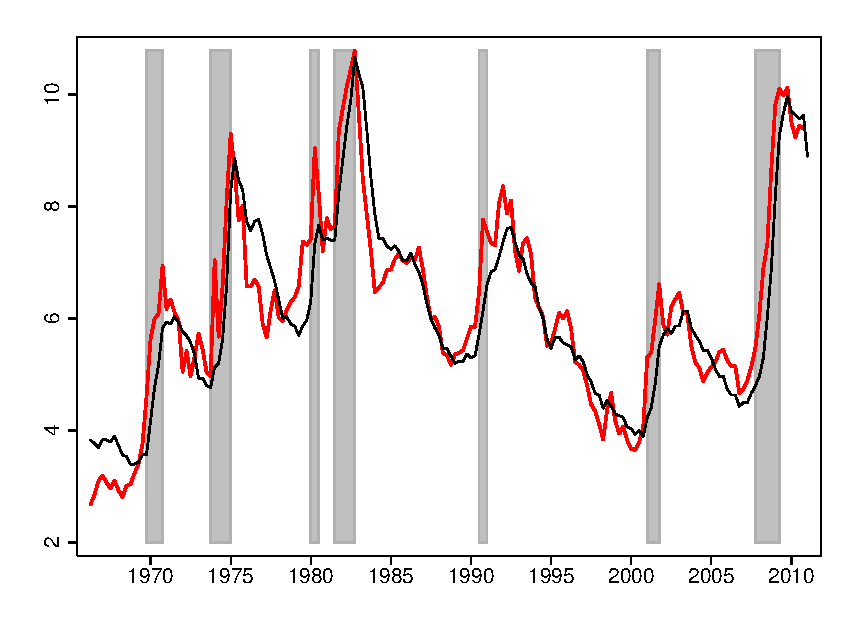
\includegraphics{\econtexRoot/Figures/mhoUnem}
%\end{center}
\footnotesize
Legend: Unemployment rate: Thin black line, Unemployment risk $\Ex_t u_{t+4}$: Thick red/grey line. Shading---NBER recessions.\\[0mm]
\tiny Sources: Thomson Reuters/University of Michigan Surveys of Consumers, \url{http://www.sca.isr.umich.edu/main.php}, Bureau of Labor Statistics.
\end{figure}


We measure a proxy $\Ex_t u_{t+4}$ for unemployment risk $\mho_t$ using re-scaled answers to the question about the expected change in unemployment in the Thomson Reuters/University of Michigan Surveys of Consumers.%
\footnote{The relevant question is: ``How about people out of work during the coming 12 months---do you think that there will be more unemployment than now, about the same, or less?''}
In particular, we estimate $\Ex_t u_{t+4}$ using fitted values $\Delta_4 \hat{u}_{t+4}$ from the regression of the four-quarter-ahead change in unemployment rate $\Delta_4 u_{t+4}\equiv u_{t+4}-u_t$ on the answer in the survey, summarized with a balance statistic $\Uexp^{BS}_t$:
\begin{eqnarray*}
\Delta_4 u_{t+4} &=& \alpha_0+\alpha_1\Uexp^{BS}_t+\varepsilon_{t+4},\\
\Ex_t u_{t+4}&=&u_t+ \Delta_4 \hat{u}_{t+4}.
\end{eqnarray*}

The coefficient $\alpha_{1}$ is highly statistically significant (indicating that households do have substantial information about the direction of future changes in the unemployment rate).  Our $\Ex_{t} u_{t+4}$ series, which---as expected---is strongly correlated with unemployment rate and indeed precedes its dynamics, is shown in Figure~\ref{fMho}.%
\footnote{We have checked that the conclusions of our analysis essentially do not change if we replaced $\Ex_{t} u_{t+4}$ with the raw unemployment series $u_t$, but we use the former series below because it is closer to the `true' perceived labor income risk.
}


\section{Reduced-Form Saving Regressions } \label{sReducedFormRegressions}

Before proceeding to structural estimation of the model of
section~\ref{ssTractableBS} we investigate a simple reduced-form
benchmark:
\be
s_t=\gamma_1+\gamma_m m_t +\gamma_{\CEA}\CEA_t+\gamma_{Eu}\Ex_t u_{t+4}+\gamma_t\,t+\gamma'X_t+\varepsilon_t. \label{srOLS}
\ee Such a specification can be readily estimated using OLS or IV
estimators, and at a minimum can be interpreted as summarizing basic
stylized facts about the data.

\begin{figure}
\caption{The Fit of the Baseline Model and the Time Trend---Actual and Fitted PSR (Percent of Disposable Income)}
%\begin{center}
\label{fOLS_fit_time_compare}
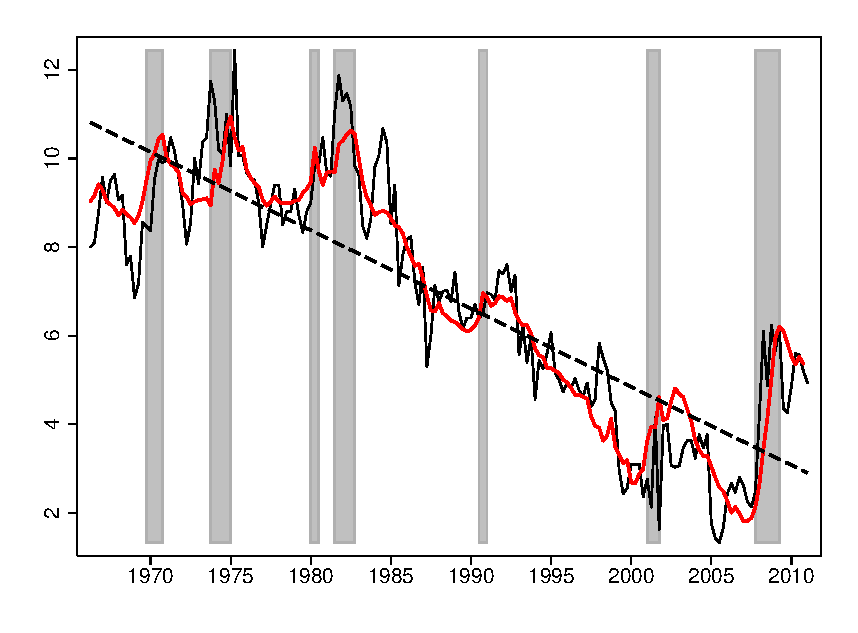
\includegraphics{\econtexRoot/Figures/fOLS_fit_time_compare}
%\end{center}
\footnotesize 
Legend: Actual PSR: Thin black line, Baseline model: Thick red/grey line, Time trend: Dashed black line. Shading---NBER recessions.\\[0mm]
\tiny Sources: Bureau of Economic Analysis, authors' calculations.
\end{figure}

\subsection{Baseline Estimates}

 Table~\ref{tOLSprelim} reports the estimated coefficients from
 several variations on equation \eqref{srOLS}.  The
 first four columns show univariate specifications in which the
 saving rate is in turn regressed on each of the three determinants
 analyzed above: wealth, credit conditions, and unemployment risk. In each specification
 we include the time trend to investigate how much each regressor
 contributes to explaining the PSR beyond the portion that can be captured mechanically
 by a linear time effect.   The three coefficients have the signs predicted
 by the model of section~\ref{ssTractableBS} and are statistically
 significant. Univariate regressions capture up to 85
 percent of variation in
 saving.%\footnote{Because the first four models only include 1--2 explanatory variables, adjusted $R^2$ and plain $R^2$ practically coincide. }

 But the univariate models on their own do not adequately describe the
 dynamics of the PSR. As the model labeled ``All 3'' in the fifth column shows, the
 three key variables of interest---wealth, credit
 conditions, and unemployment risk---jointly explain roughly 90 percent of the variation in
 the saving rate over the past five decades. As expected, the point
 estimates again indicate a strong negative correlation between saving
 and net wealth and credit conditions and a positive correlation with
 unemployment risk. Interestingly, once the three variables are
 included jointly, the time trend ceases to be significant, which is
 in line with the fact that the three models in columns 2--4 have
 higher $\bar{R}^2$ than the univariate model with the time trend
 only.%
 \footnote{   Estimating univariate saving regressions without the time trend
   results in higher $\bar{R}^2$ for wealth and the credit
   conditions---0.72 and 0.80, respectively---than for the ``time''
   model in column one (0.70). (Because unemployment risk is not
   trending, it captures relatively little variation in saving on its
   own (about 10 percent) but is important \emph{in addition} to the
   two other factors, as illustrated in columns 4 and 5.)  }

 A more parsimonious version of the model without the time trend reported in column
 6 (Baseline)---as also suggested by the model in
 section~\ref{ssTractableBS}---neatly summarizes the key features of
 the saving rate.  The estimated coefficient on net wealth implies the
 (direct) long-run marginal propensity to consume of about 1.2 cents out
 of a dollar of (total) wealth. The value is low compared
 to much of the literature, which typically estimates a marginal
 propensity to consume out of wealth (MPCW) of about 3--7 cents
 without explicitly accounting for credit conditions.%
 \footnote{   See, for example, \cite{skinner96_sideshow},
   \cite{ludvigsonSteindel_99}, \cite{llTrendCycle}, \cite{cqs05}, and
   \cite{cos11}. See \citet{mue07} and \cite{ducaEtAl10_creditArch}
   for a model which includes a measure of credit conditions in the
   consumption function.  } However, a univariate model regressing
 the PSR just on net wealth (not reported here), implies an MPCW of
 4.3 percent.  These results suggest that much of what has been interpreted as pure ``wealth effects'' in the prior literature may actually have reflected precautionary or credit availability effects that are correlated with wealth.

The coefficient on the Credit Easing Accumulated index is highly
statistically significant with a $t$ statistic
of
\input{./Tables/results/CEAtstat_base.tex}. The point estimate of $\gamma _{\CEA}$ implies that increased
access to credit over the sample period until the Great Recession
reduced the PSR by about 6 percentage points of disposable income. In
the aftermath of the Recession, the \CEA\ index declined between 2007 and
2010 by roughly \input./Tables/results/dCEA.tex
as credit supply tightened, contributing roughly \input./Tables/results/CEATimesdCEA.tex
 percentage point to the increase in the PSR (see the discussion of Table~\ref{tPred} below for more detail).

Figure~\ref{fOLS_fit_time_compare} further illustrates why we find the
``baseline'' specification in column 6 more appealing than the more
atheoretical model with a linear time trend. The trends in saving and
the \CEA\ are both non-linear, moving consistently with each other
even within our sample and often persistently departing from the
linear trend (as indicated by the time-only model's substantially lower
$\bar{R}^2$).  In addition, it is likely that the time-only model will
become increasingly problematic as observations beyond our sample
accumulate, arguably providing additional evidence on a possible structural
break in the time model during the Great Recession.%
\footnote{  Reliable PSR data only start in 1959 and document that the downward
  trend in saving started around 1975, so that our sample is actually
  quite favorable to the time-only model; it would have considerably more
difficulty with a sample that included 10 pre-sample years without a discernable
trend.}

Finally, the last model investigates the joint effect of credit conditions
and unemployment risk. The structural model of section~\ref{ssTractableBS}
implies that uncertainty affects saving more strongly when credit
constraints bind tightly; the model in column 7 (Interact) confirms the prediction with a (borderline) significant negative interaction term between the \CEA\ and unemployment risk.%
\footnote{  Adding an interaction term between the \CEA\ and wealth results in a
  borderline significant positive estimate, which is in line with the
  concavity of the consumption function, show in
  Figure~\ref{fig:PhaseDiag}.  }

\subsection{Robustness Checks}

Table~\ref{tOLS} presents a second battery of specification checks of
the baseline model shown again for reference as the first `model.'  The second model (Uncertainty) investigates the effects of adding to the baseline regression an
alternative proxy for uncertainty: the
\cite{bloomFloetottoJaimovich_rubc} index of macroeconomic and
financial uncertainty.%
\footnote{See \cite{baker_policyUncertainty} for related work measuring \emph{economic policy} uncertainty.
}
 The new variable is statistically insignificant
and the coefficients on the previously included variables are broadly
unchanged, suggesting that our baseline uncertainty measure is more
appropriate for our purposes (which makes sense, as personal saving is
conducted by persons, whose uncertainty is likely better captured by
our measure of labor income uncertainty than by the
\cite{bloomFloetottoJaimovich_rubc} measure of firm-level shocks).

The third model (Lagged $s_{t-1}$) explores the implications of adding lagged saving to the list of regressors.  Often in empirical
macroeconomics, the addition of the lagged dependent variable is unjustified by the underlying theory, but nevertheless is required
for the model to fit the data.  Here, however, serial correlation in saving is a direct implication of the model (below we will show that the degree of serial correlation implied by the model matches the empirical estimate fairly well).  The implication arises because deviations of actual wealth from target wealth ought to be long-lasting if the saving rate cannot quickly move actual wealth to the target.  As expected, the coefficient is highly statistically significant.  However, this positive autocorrelation only captures near-term stickiness and has little effect on the long-run dynamics of saving. Indeed, the coefficients from the baseline roughly equal their long-term counterparts from the model with lagged saving rates (that is, coefficient estimates pre-multiplied by $2.5$, or $1/(1-\gamma_s)=1/(1-0.60)$).\footnote{Note that with the inclusion
  of lagged saving, the Durbin--Watson statistic becomes close to 2,
  suggesting that whatever serial correlation exists in the
  other specifications reflect simple first order autocorrelation of
  the errors.}

The fourth model (Debt) explores the role of the debt--income ratio. The variable could be relevant for two reasons. First, it could partly account for the fact that debt is held by a different group of people than assets and consequently net worth might be an insufficient proxy for wealth. Second, debt might also reflect credit conditions (although---as mentioned above---we prefer the CEA index because in principle it isolates the role of credit supply from demand). The regression can thus also be interpreted as a horse-race between the CEA and the debt--income ratio. In any case, while the coefficient $\gamma_d$ has the correct (negative) sign, it is statistically insignificant and its inclusion does not substantially affect estimates obtained under the baseline specification.


\begin{figure}
\caption{The Fit of the Baseline Model and the Model with Full Controls (of Table~\ref{tOLS})---Actual and Fitted PSR (Percent of Disposable Income)}
%\begin{center}
\label{fFullControls}
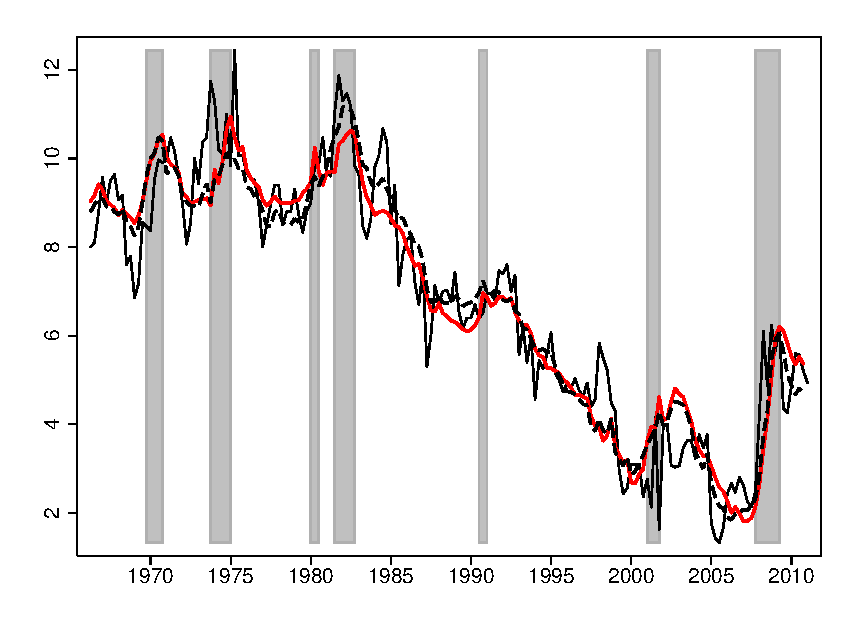
\includegraphics{\econtexRoot/Figures/fFullControls}
%\end{center}
\footnotesize
Legend: Actual PSR: Thin black line, Baseline model: Thick red/grey line, Model with full control variables: Dashed black line. Shading---NBER recessions.\\[0mm]
\tiny Sources: Bureau of Economic Analysis, authors' calculations.
\end{figure}
%\small
%Notes: Shading---NBER recessions.\\[0mm]


The fifth model (Multiple Controls) controls for the effects of several other potential determinants of
household saving: expected real interest rates, expected income
growth, and government and corporate saving (both measured as a
percent of GDP).%
\footnote{  Expected real interest rates and expected income growth are
  constructed using data from the Survey of Professional Forecasters
  of the Philadelphia Fed.} Some of these factors are statistically
significant, but all are inconsequential in economic
terms. A plot of fitted values in Figure~\ref{fFullControls} makes it clear that while these
additional factors were potentially important during specific episodes
(especially in the early 1980s), they have on average had only a
limited impact on U.S.\ household saving. The negative coefficient on
corporate saving is consistent with the proposition that households
may `pierce the corporate veil' to some
extent\footnote{Regressions with total private saving as a dependent
  variable yield qualitatively similar results as our baseline
  estimates in Table~\ref{tOLSprelim}.  } but there is no evidence for
any interaction between personal and government saving.  One
interpretation of this is that `Ricardian' effects that some prior
researchers have claimed to find might instead reflect reverse
causality: Recessions cause government saving to decline at the same
time that personal saving increases (high unemployment, falling
wealth, restricted credit) but for reasons independent of the Ricardian
logic (reduced tax revenues and increased spending on automatic
stabilizers, e.g.).  Since we are controlling directly for the variables
(wealth, unemployment risk, credit availability) that were (in this
interpretation) proxied by government saving, we no longer find any effect
of government saving on personal saving.

The sixth model (Income Inequality) explores the idea that growing income inequality
 has resulted in an increase in the aggregate saving rate, to the extent that microeconomic evidence
 points to high personal saving rates among the higher-permanent-income households
 (\cite{carroll:richsave}; \cite{dszRichSave}). However, the econometric evidence is mixed.
 We have experimented with numerous income inequality series of \cite{Piketty_Saez2003} (updated through 2010)
 in our regressions: we included income shares of the top 10, 5, 1, 0.5, and 0.1 percent of the income distribution,
 either with or without capital gains. None of these 10 series were statistically significant in the full 1960--2010
 sample; one of the estimated specifications is reported in Table~\ref{tOLS}. Some of the inequality measures
 were statistically significant in a shorter, 1980--2010, sample. In this specific sub-sample (results not reported here),
 the coefficients on credit conditions and net wealth remained highly statistically significant, although the coefficient
 on credit conditions tended to be more negative than in the baseline specification. The coefficient on unemployment expectations
 became insignificant, which is also natural since income inequality fluctuates over the business cycle.

The seventh model (DB Pensions) examines whether the shift from defined benefit to defined contribution pension plans
 may also have had a measurable effect on the aggregate saving rate. Aggregate data on the size of defined-benefits pension
 plans are not readily available; the NIPA provides the relevant series only since 1988. As an initial experiment,
 we calculated the share of employer contributions accruing to the defined benefit plans as a percent of total contributions;
 however, this variable was not statistically significant in our regressions (sample 1988--2010). As an alternative, we compiled
 a measure of household saving adjusted for the defined-benefit pension plans from various research publications
 by the Bureau of Economic Analysis (BEA; \cite{kmitchSaving}, \cite{prSaving}) and Congressional Budget Office (CBO; \cite{CBOSaving}). Subsequently, we calculated ``a pension gap,'' defined as the difference between the headline saving rate
 and the BEA/CBO adjusted saving rate, and included this gap variable in our regressions (sample: 1960--2007). The gap is statistically
 significant with a coefficient of about 0.7. This suggests that the shift from defined benefit to defined contribution pension plans
 may have reduced the aggregate saving rate. However, this effect appears small in economic terms: the contribution of the changing pension system
 to the overall decline in the saving rate since the 1980s is only about 1 percentage point of disposable income. The coefficients on the baseline series (credit conditions, net wealth, unemployment expectations) remain highly statistically significant in this regression.

The eighth and ninth models (High Tax Bracket and Low Tax Bracket) provide a first-pass test of the effects of tax policy
 on aggregate saving by including the data on the highest and lowest marginal tax rates in our regressions. Neither of the two
 variables are statistically significant.


Finally, to explore how much endogeneity may matter,%
\footnote{As mentioned above, wealth is lagged by one quarter to alleviate
  endogeneity in OLS regressions.  However, a standard concern about reduced-form regressions like \eqref{srOLS} is that the OLS coefficient estimates might be biased because the regressions do not adequately account for all relevant right-hand size variables (such as expectations about income growth; see also Appendix~2 for further discussion).
  }
  the specification ``IV'' re-estimates
the baseline specification using the IV estimator. Instruments are
the lags of net wealth, unemployment risk and---crucially---the Financial Liberalization Index of \cite{abiadEtAl_FinReforms} (described in Appendix~1).
The FLI is an alternative measure of credit conditions constructed using the records about legal and regulatory changes in the banking sector. The index intends to capture exogenous changes in credit conditions. While it is a rough approximation as it reflects only the most important events (see also Figure~\ref{fCreditAvailability} in Appendix~1), the profile of the FLI matches well that of the CEA. The
estimated coefficients remain broadly unchanged compared with the baseline specification.

We have also estimated specifications with other potential determinants of saving, whose
detailed results we do not report here. As in
\citet{parker_nberma_spendthrift}, variables capturing demographic trends such as the
old-age dependency ratio were insignificant in our regressions. The
importance of population aging in cross--country studies of household
saving (for example, \cite{bloomEtAl_JME07} and
\cite{bosworthChodorowReich07}) appears to be largely driven by the
experience of Japan and Korea---countries well ahead of the United
States in the population aging process.

\subsection{Sub-Sample Stability}

When the model is estimated only using the post-1980 data in Table~\ref{tOLS_subSample}
(Post-1980), its fit measured by the $\bar{R}^2$ actually
improves, in contrast with many other economic relationships,  % (e.g., the Phillips curve; \cite{stockWatson_pieHarderForecast_jmcb07} and \cite{stockWatson_pcFore},
 whose goodness-of-fit deteriorated in the past 20 years.
 The F test does not reject the proposition that the regression coefficients have remained stable over the sample period. Allowing for a structural break at the start of the Great Recession in 2007q4 (column `Pre-2008') does not affect much the baseline estimates. (The estimated values of the post-2007 interaction dummies and their standard errors are of course not particularly meaningful because the relevant sub-sample only consists of 13 observations.)

To address the potential criticism that saving rate regressions are
difficult to interpret because aggregate income shocks reflect a mix
of transitory and persistent factors, we have also re-estimated our
regressions with alternative measures of disposable income (see
Appendix 2) which exclude a range of identifiable temporary shocks
such as fiscal stimulus and extreme weather. There was little
econometric evidence that transitory movements in aggregate disposable
income are substantial and our econometric results basically did not
change.\footnote{Interestingly, an auxiliary regression of income
  growth on the lagged saving rate in the spirit of \cite{cam87}
  yields statistically insignificant slope when post-1985 data are
  included (see Table~\ref{tCampbell87} in Appendix~2).  }

\subsection{Saving Rate Decompositions}

Table~\ref{tPred} reports an in-sample fit of the baseline model and
the model Interact with the \CEA--uncertainty interaction term of
Table~\ref{tOLSprelim}, together with the contributions of the individual
variables to the explained increase in the saving rate between 2007
and 2010. Two principal conclusions emerge. First, both models
(especially the latter) are able to capture well the observed change
in the saving rate. Second, the key explanatory factors in saving were the changes in wealth and uncertainty, with
credit conditions (as measured by \CEA) playing a less important role.  While the
change in the trajectory of the \CEA\ index is quite striking (see
Figure~\ref{fCEA}), and may explain the sudden academic interest in the
role of household credit over the business cycle (see the papers cited
in the introduction), this evidence suggests that the rise in saving
cannot be primarily attributed to the decline in credit availability.  If
correct, this finding is particularly important at the present
juncture because it suggests that however much the health of the
financial sector continues improving, the saving rate is likely to remain high so
long as uncertainty remains high and household wealth remains impaired
(compared, at least, to its previous heights).

\section{Structural Estimation} \label{sStructuralEstimation}

This section estimates the structural model of section~\ref{ssTractableBS} by minimizing the distance between the data on saving implied by the model and the corresponding empirical data. The nonlinear least squares (NLLS) procedure employed here has some advantages over the reduced-form regressions. Besides arguably being more immune to endogeneity and suitable for estimating structural parameters (such as the discount factor), it imposes on the data a structure that makes the parameter values easier to interpret. As Figure~\ref{fig:PhaseDiag} documents, the structural model also explicitly justifies and disciplines non-linearities, which can be important especially during turbulent times, when the shocks are large enough to move the system far from its steady state.

\subsection{Estimation Procedure}

We assume households instantaneously observe exogenous movements in
three variables: wealth shocks $\mRat$, unemployment risk $\mho$ and
credit supply conditions $\CEA$, and that they consider the shocks to
$\mho$ and $\CEA$ to be permanent, and do not expect the shocks to
wealth to be reversed.\footnote{The assumption that households
  believe the shocks to be permanent is necessary for us to be able to
  use the tractable model we described earlier in the paper.  While
  indefensible as a literal proposition (presumably nobody believes
  the unemployment rate will remain high forever), the high serial
  correlation of these variables means that the assumption may not be
  too objectionable.  In any case, a model that incorporated more
  realistic descriptions of these processes would be much less
  transparent and might not be computationally feasible with present
  technology.} Given these observables, consumers
re-optimize their consumption--saving choice in each period. Collecting the parameters in vector
$\Theta$ and denoting the target wealth $\check{\mRat}_t(\cdot)$ and
the corresponding wealth gap $\mRat_t-\check{\mRat}_t$, the model
implies a series of saving rates $s_t^{\text{theor}}(\Theta;
m_t-\check{\mRat}_t)$, which we match to those observed in the data,
$s_t^{\text{meas}}$. Our estimates of $\hat{\Theta}$ thus solve the
following problem: \be \hat{\Theta}=\argmin
\sum_{t=1}^T\bigg(s_{t}^{\text{meas}}-s_t^{\text{theor}}\Big(\Theta;
\mRat_t-\check{\mRat}\big(\underline{h}(\CEA_t),\mho(\Ex_tu_{t+4})\big)\Big)\bigg)^2, \label{minDist}
\ee where the target wealth $\check{\mRat}$ depends on the credit
conditions and unemployment risk as described in
section~\ref{ssTractableBS}. In our baseline specification, the
parameter vector $\Theta$ consists of the discount factor $\Discount$
and the scaling constants for credit conditions and unemployment risk:
\begin{eqnarray}
\Theta&=&\{\Discount,\bar{\theta}_h,\theta_\CEA,\bar{\theta}_\mho,\theta_u\},\\
\underline{h}_t&=&\bar{\theta}_h+\theta_\CEA \CEA_t, \\
\mho_t&=&\bar{\theta}_\mho+\theta_u \Ex_tu_{t+4}.
\end{eqnarray}
The re-scaling ensures that the unitless measure of credit conditions is re-normalized as a fraction of disposable income and that the expected unemployment rate is transformed into the model-compatible equivalent of \emph{permanent} risk. The model implies that $\theta_\CEA>0$ and $\theta_u>0$.

Minimization \eqref{minDist} is a non-linear least squares problem for which the standard asymptotic results apply. Standard errors for the estimated parameters are calculated using the delta method as follows.%
\footnote{To construct the objective function (which we then minimize over $\Theta$) we need to solve the consumer's optimization for each quarter. Because the calculation is computationally demanding, we cannot apply bootstrap to calculate standard errors. (The Shapiro--Wilk test does not reject normality of residuals.)
}
Define the scores $q_t(\Theta)=\big(s_{t}^{\text{meas}}-s_t^{\text{theor}}(\Theta)\big)\frac{\partial s_t^{\text{theor}}(\Theta)}{\partial \Theta'}$ and the $5\times5$ matrices $E=\var\big(q_t(\Theta)\big)$ and $D=\Ex\frac{\partial q_t(\Theta)}{\partial \Theta'}$. The estimates have the asymptotic distribution:
$$
T^{1/2}(\hat{\Theta}-\Theta)\rightarrow_d \mathscr{N}(0, D^{-1}ED'^{-1}).
$$
Because the saving function $s_t^{\text{theor}}(\Theta)$ is not available in the closed form, we calculate its partial derivatives numerically.

\subsection{Results}

Table~\ref{tStructEst} summarizes the calibration and estimation results. The calibrated parameters---real interest rate $\rfree=0.04/4$, wage growth $\Delta\Wage=0.01/4$ and the coefficient of relative risk aversion $\CRRA=2$ take on their standard quarterly values and meet (together with the discount factor $\Discount$) the conditions sufficient for the problem to be well-defined.

The estimated discount factor $\Discount=1-0.0064=0.9936$, or $0.975$ at annual frequency, lies in the standard range.
Figure~\ref{tMbar} shows the estimated horizontal shift in the consumption function $\underline{h}_t$. The estimates of the scaling factors $\bar{\theta}_h$ and ${\theta}_\CEA$ imply that $\underline{h}_t$ varies between $0.88/4\approx0.2$ and $(0.88+5.25/4)\approx1.5$, implying that financial deregulation resulted at its peak in an availability of credit in 2007 that was greater than credit availability at the beginning of our sample in 1966 by an amount equal to about 130\%\ of annual income---not an unreasonable figure (note that this figure should not be compared with the aggregate debt ratio, which peaked at around 135 percent of disposable income, but with the total amount of net wealth which is substantially higher).
Figure~\ref{tMhoRescaled} shows the estimated quarterly intensity of perceived permanent unemployment risk.


\begin{figure}
\caption{Extent of Credit Constraints $\underline{h}_t$ (Fraction of Quarterly Disposable Income) \label{tMbar}}
%\begin{center}
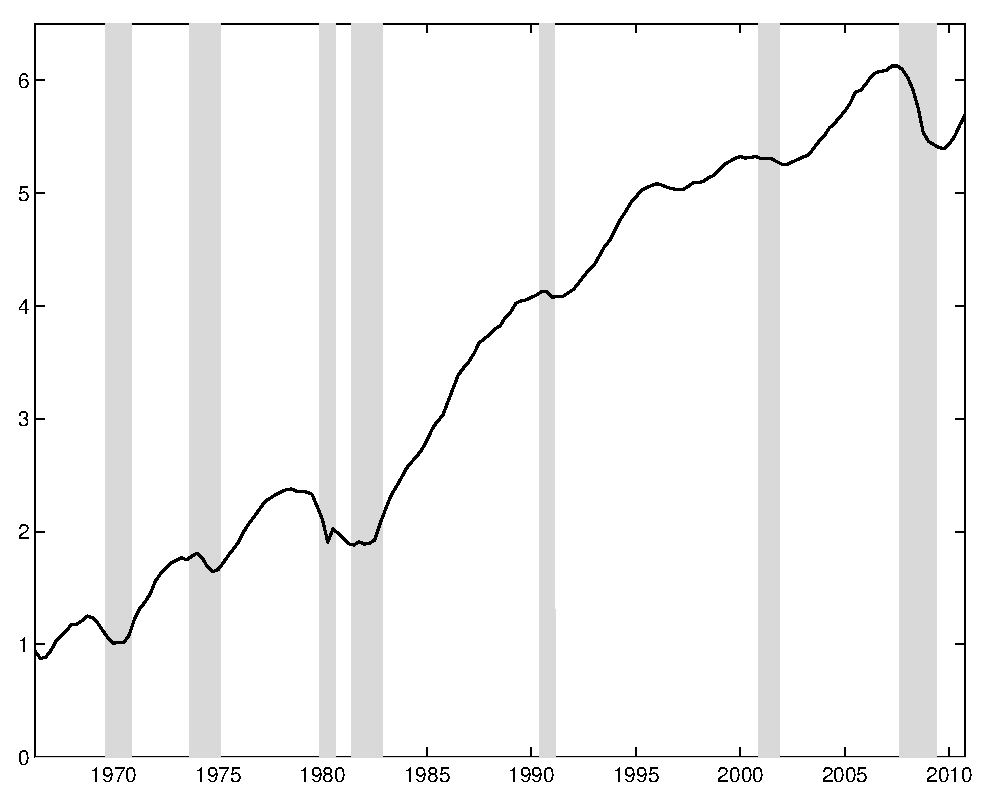
\includegraphics{\econtexRoot/Figures/fCEA_est}
%\end{center}
\footnotesize
Notes: Shading---NBER recessions.\\[0mm]
\tiny Sources: Federal Reserve, accumulated scores from the question on change in the banks' willingness to provide consumer installment loans from the Senior Loan Officer Opinion Survey on Bank Lending Practices, \url{http://www.federalreserve.gov/boarddocs/snloansurvey/}, authors' calculations.
\end{figure}

\begin{figure}
\caption{Per Quarter Permanent Unemployment Risk $\mho_t$  \label{tMhoRescaled}}
%\begin{center}
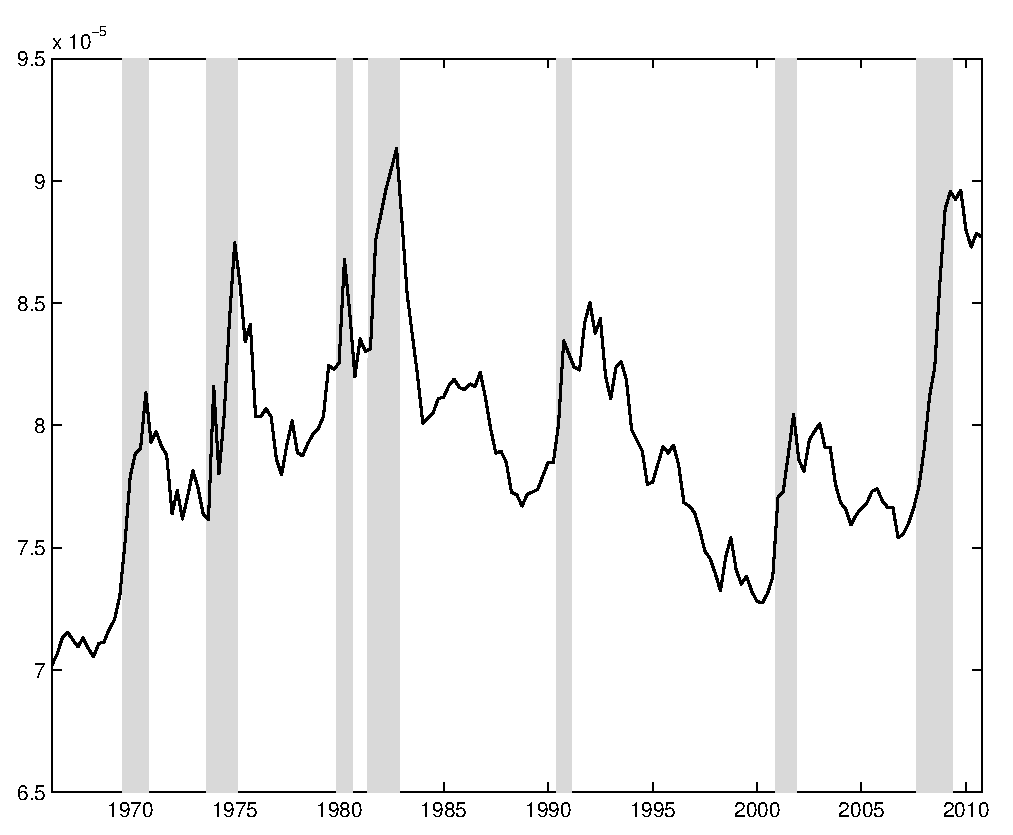
\includegraphics{\econtexRoot/Figures/fMho_est}
%\end{center}
\footnotesize
Notes: Shading---NBER recessions.\\[0mm]
\tiny Sources: Thomson Reuters/University of Michigan Surveys of Consumers, \url{http://www.sca.isr.umich.edu/main.php}, Bureau of Labor Statistics, authors' calculations.
\end{figure}

\begin{comment} % CDC: I think this is more confusing than illuminating, so have removed it.  We're already showing the consumption function in the phase diagrams, and everybody knows that (a) consumption is lower in the presence of a precautionary motive; (b) it's concave; and (c) without the precautionary motive it's linear
Figure~\ref{fEstCfunction} shows the estimated consumption function of section~\ref{ssTractableBS} and its linear counterpart, which governs the spending of a consumer with perfect foresight. The vertical distance between the two functions gives the extent of precautionary saving, which is quite substantial. For example, for the wealth--disposable income ratio of 20 (the sample mean)
% Jirka: Note: mean labor/disposable income ratio in our sample = 0.625
precautionary saving makes up roughly 11 percent of disposable income.
% Chris: Please decide if we want to keep the 11 percent in the paper (if it's not confusing to the reader).

\begin{figure}
\caption{Estimated Consumption Functions Under Uncertainty and Under Perfect Foresight \label{fEstCfunction}}
%\begin{center}
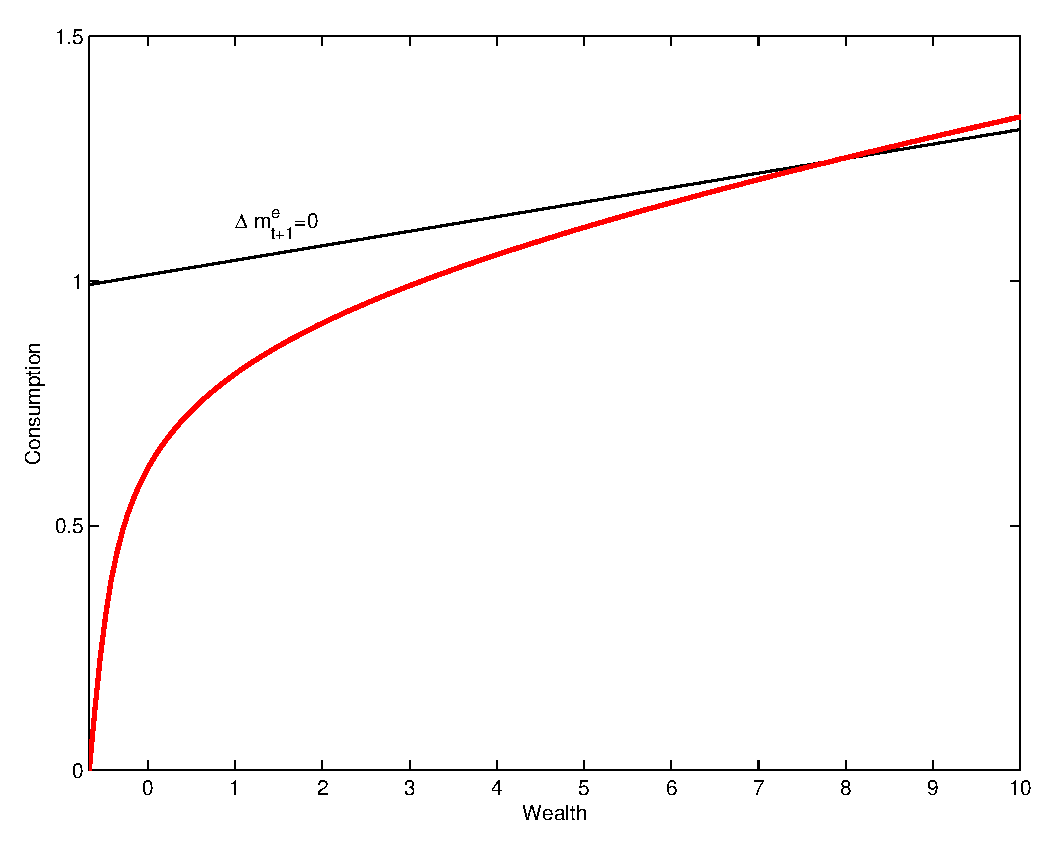
\includegraphics{\econtexRoot/Figures/fEstCfunction}
%\end{center}
\footnotesize
Legend: Perfect Foresight Consumption Function: Thin black line, Consumption Function Under Uncertainty: Thick red/grey line.\\
The two consumption functions are calibrated using parameters from the top panel of Table~\ref{tStructEst}. The concave consumption function also assumes that  $\underline{h}=0$ and uncertainty is at its sample mean $\mho=\bar{\mho}_t=6.8\times10^{-5}$.
\\[0mm]
\end{figure}
\end{comment}

%Figure~\ref{fPrecSav} shows that precautionary saving (calculated as the vertical distance between the consumption function under uncertainty and under perfect foresight) is counter-cyclical. Both the (pro-cyclical) shocks to wealth and by the counter-cyclical labor market risk $\mho_t$ contribute to the counter-cyclicality of precautionary saving.

%\begin{figure}
%\caption{Precautionary Saving over the Business Cycle \label{fPrecSav}}
%\begin{center}
%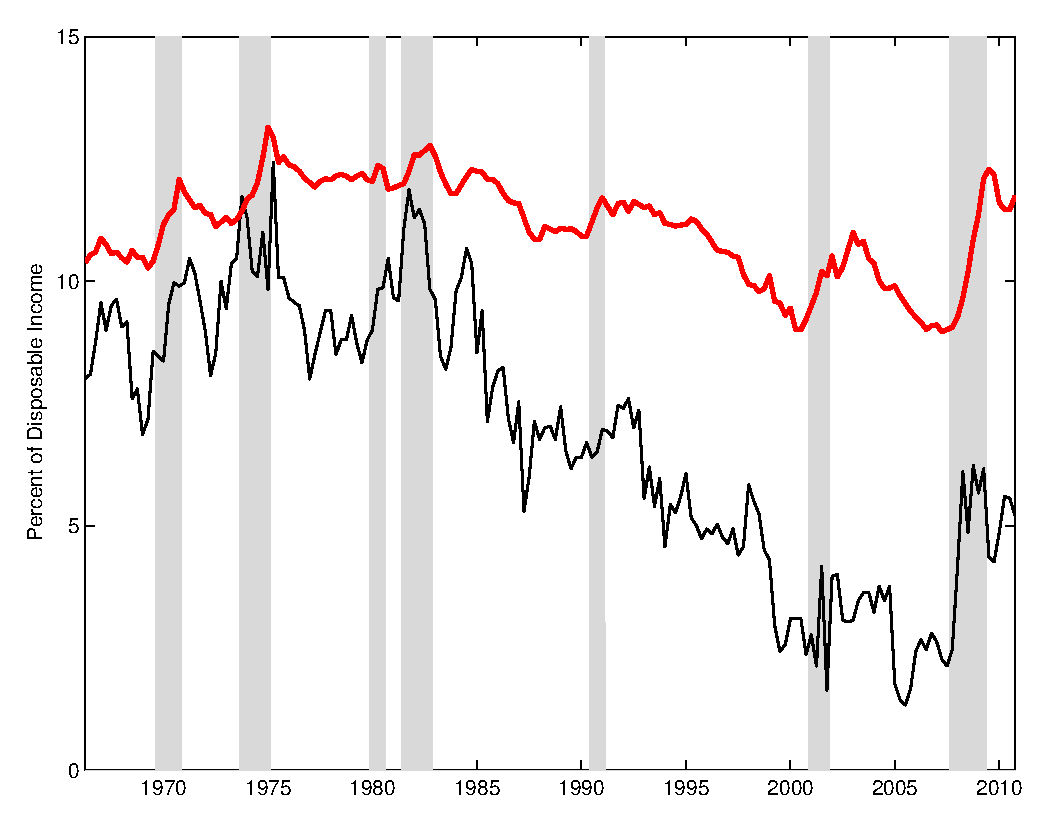
\includegraphics{\econtexRoot/Figures/fPrecSav}
%\end{center}
%\small
%Legend: Actual PSR: Thin black line, Precautionary Saving: Thick red/grey line. Shading---NBER recessions.\\[0mm]
%Sources: Bureau of Economic Analysis, authors' calculations.\\[0mm]
%\end{figure}

Figure~\ref{fPSR_StructFit} shows the fit of the structural model. In terms of $\bar{R}^2$ (Table~\ref{tStructEst}), the model captures more than 80 percent of variation in the saving rate, doing only slightly worse than our baseline reduced-form model (whose $\bar{R}^2$ is roughly 0.9). The Mincer--Zarnowitz horse race between the models puts weight of 0.72 on the structural model. % (although the high standard error on the coefficient signals the high correlation between the two model-implied saving rates).

\begin{figure}
\caption{Fit of the Structural Model---Actual and Fitted PSR (Percent of Disposable Income) \label{fPSR_StructFit}}
%\begin{center}
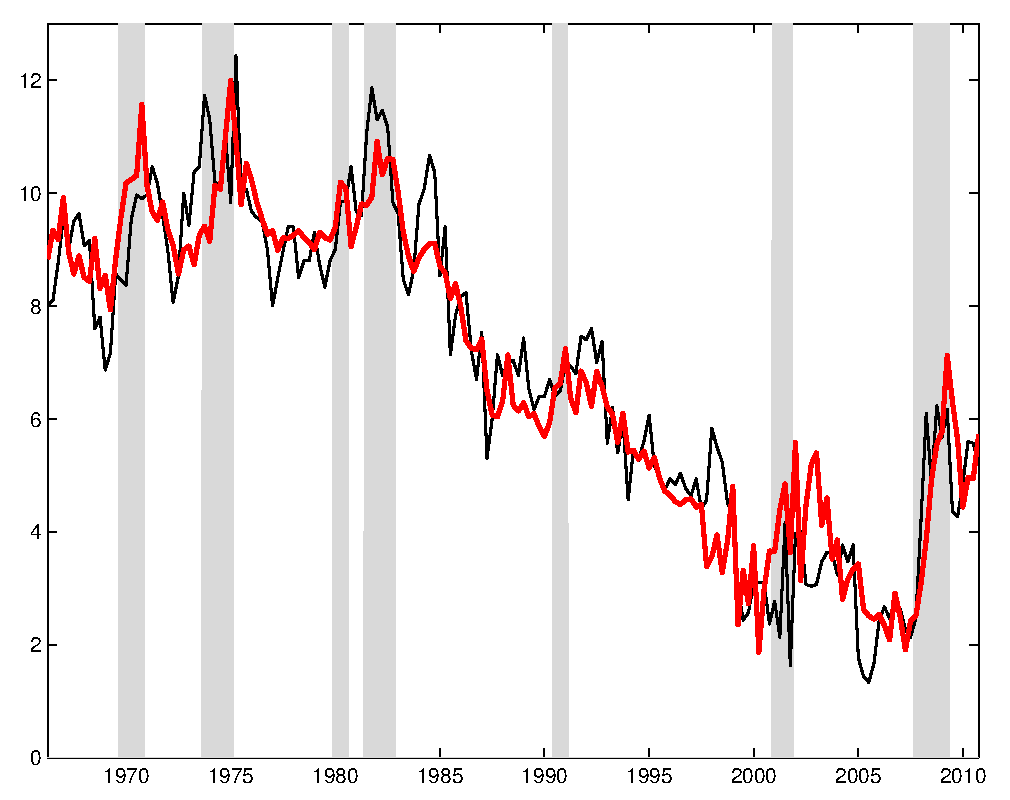
\includegraphics{\econtexRoot/Figures/fPSR_StructFit}
%\end{center}
\footnotesize
Legend: Actual PSR: Thin black line, Structural model: Thick red/grey line. Shading---NBER recessions.\\[0mm]
\tiny Sources: Bureau of Economic Analysis, authors' calculations.
\end{figure}

In principle, time variation in the fitted saving rate arises as a result of movements in its three time-varying determinants: uncertainty, wealth, and credit conditions, see Figure~\ref{fPSR_StructDecomp}. To gauge the relative importance of the three main explanatory variables, we sequentially switch off the uncertainty and credit supply channels by setting the values of these series equal to their sample means. Note that the difference between the fitted series  (red/grey line) and the fitted series excluding uncertainty (black line) should be interpreted as the effect of \emph{time variation} in unemployment risk $\mho$ rather than the \emph{total amount} of saving attributable to uncertainty. The main takeaway from the Figure is that the CEA is essential in capturing the trend decline in the PSR between the 1980s and the early 2000s. The wealth fluctuations contribute to a good fit of the model at the business-cycle frequencies, and the principal role of cyclical fluctuations in uncertainty is to magnify the increases in the PSR during recessions.

\begin{figure}
\caption{Decomposition of Fitted PSR  (Percent of Disposable Income) \label{fPSR_StructDecomp}}
%\begin{center}
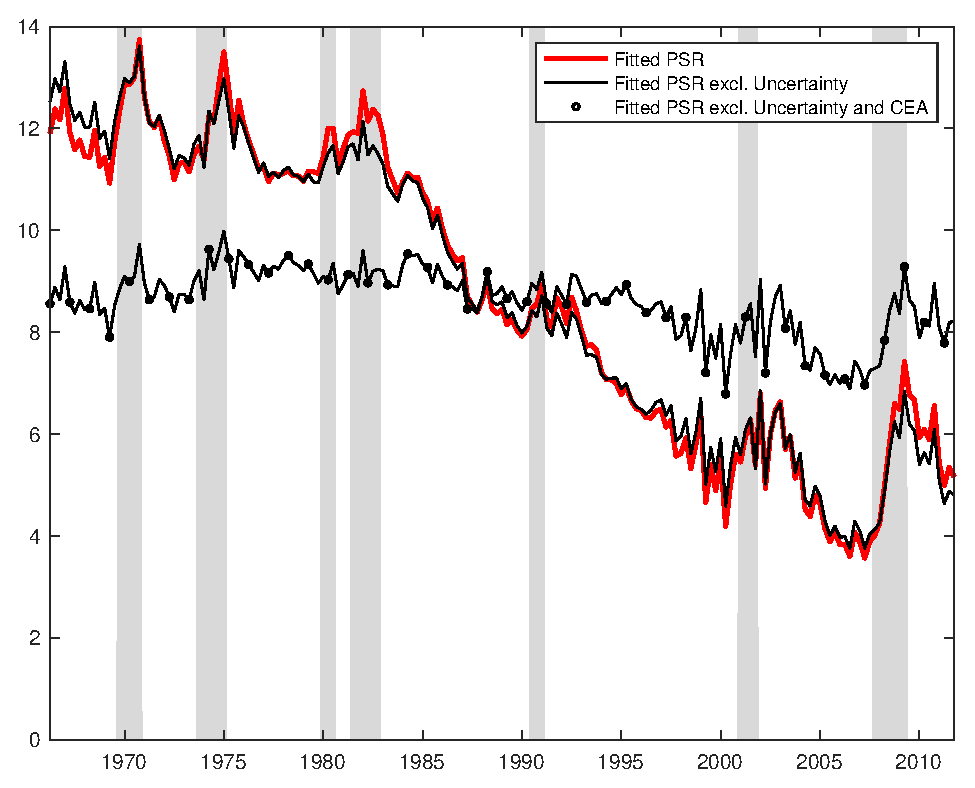
\includegraphics{\econtexRoot/Figures/fPSR_StructDecomp}
\footnotesize
Notes: Shading---NBER recessions.\\[0mm]
\tiny Sources: Bureau of Economic Analysis, authors' calculations.
\end{figure}

Table~\ref{tOLSprelim_model} replicates the estimates of Table~\ref{tOLSprelim} for the artificial saving series generated by the estimated structural model. The coefficient estimates closely mirror those obtained from actual data which means that the structural model captures well the key features of the saving data. Unsurprisingly, the standard errors are somewhat smaller than those in Table~\ref{tOLSprelim} and the $\bar{R}^2$s are higher because the process of generating artificial data by the model eliminates much of the noise present in the actual PSR data.



\section{Conclusions}

We find evidence that credit availability, shocks to household wealth, and movements in income uncertainty proxied by unemployment risk have all been important factors in driving U.S.\ household saving over the past 45 years. In particular, the relentless expansion of credit supply between the early-1980s and 2007 (likely largely reflecting financial innovation and liberalization), along with higher asset values and consequent increases in net wealth (possibly also partly attributable to the credit boom) encouraged households to save less out of their disposable income. At the same time, the fluctuations in net wealth and labor income uncertainty, for instance during and after the burst of the information technology and credit bubbles of 2001 and 2007, can explain the bulk of business cycle fluctuations in personal saving.

We also find that other determinants of saving suggested by various literatures (e.g.,
fiscal deficits, demographics, income expectations) either work
through the key factors above, are of second-order importance, or
matter only during particular episodes. These findings are broadly in
line with the complementary household-level evidence reported in
\cite{dynanKohn07_indebtedness},
\cite{moorePalumbo_financesOfUShouseholds},
\cite{brickerEtAl_storm}, \cite{mianRaoSufi_hhBalanceSheets} and \cite{petevEtAl_cAndGreatRecession}.%
\footnote{  \cite{dynanKohn07_indebtedness} find that data from the Federal
  Reserve's Survey of Consumer Finances (SCF) and the Michigan Survey
  of Consumer Sentiment show too little variation in the measures of
  impatience, risk aversion, expected income, interest rates and
  demographics to adequately explain the household indebtedness. In
  contrast, they argue that house prices and financial innovation have
  been important drivers of
  indebtedness. \cite{moorePalumbo_financesOfUShouseholds} document
  that the drop in consumer spending during the Great Recession was
  accompanied by significant erosions of home and corporate equity
  held by households. Using SCF data, \cite{brickerEtAl_storm}
  document higher desired precautionary saving among most families
  during the Great Recession.  \cite{mianRaoSufi_hhBalanceSheets} use county- and zip-code-level data
  to document that the recent decline in consumption was much stronger in high leverage counties with large house prices declines.
  \cite{petevEtAl_cAndGreatRecession} discuss the following factors
  behind the observed changes in consumption during the Great Recession: the wealth effect, an increase in uncertainty and the credit crunch.
  \cite{dynan_debtOverhang} finds that highly indebted households cut spending more strongly that their less-indebted counterparts despite
  experiencing smaller declines in net worth.
  }

There can be little doubt that factors aside from those which are the primary focus in our model have had some effect on U.S.\ saving dynamics over our sample
period.  For example, \cite{ssModeration} show a substantial decline in the size of both transitory and permanent shocks to income over the past 40 years;
 this should have led to a decline in precautionary saving that is probably not fully captured by the fact that our measure
 of unemployment risk is only somewhat lower in the latter than in the earlier part of our sample.  Despite our extensive robustness checks reported
 in Table~\ref{tOLS}, factors such as the shift from defined benefit to defined contribution pension plans, changing rates of taxation,
 or the large increase in income inequality that has taken place since the mid-1970s might have played a more important role than suggested
 by our regressions due to difficult-to-tackle measurement issues. Real progress on such questions will likely require the use of good ``natural experiments'' in a microeconomic setting.

Finally, it is worth keeping in mind that our econometric evidence is based on historical data and, going
forward, factors such as rapidly rising federal debt or the retirement
of baby-boomers could yet lead to new structural shifts in household
saving. But our results suggest that the personal saving rate in the
pre-crisis period was artificially low because of the bubble in
housing prices and the corresponding easy availability of credit.
Neither of these factors are likely to return soon, and since
consensus forecasts suggest that the unemployment rate may
remain elevated for a long time, there seems to be little prospect
that the personal saving rate could return to its low pre-crisis value
anytime in the foreseeable future.

% More research is needed in the future to understand the determinants of credit conditions and the linkages between credit conditions and asset prices.

%Other variables beside credit availability and the wealth gap contribute to the dynamics of the saving rate only a little or not at all. While we know from theoretical models that expected interest rate, expected income growth, demographics, or government savings can have large effect on the PSR, these variables have varied either too little or not consistently enough to be able to capture the movements in the PSR.


\small

%\input{\econtexBibMake}
\bibliography{economics,\econtexRoot/cssUSSaving,\econtexRoot/cssUSSaving-Add}


\clearpage
\section*{Appendix 1: Comparison of Alternative Measures of Credit Availability}


\begin{figure}
\caption{Alternative Measures of Credit Availability \label{fCreditAvailability}}
%\begin{center}
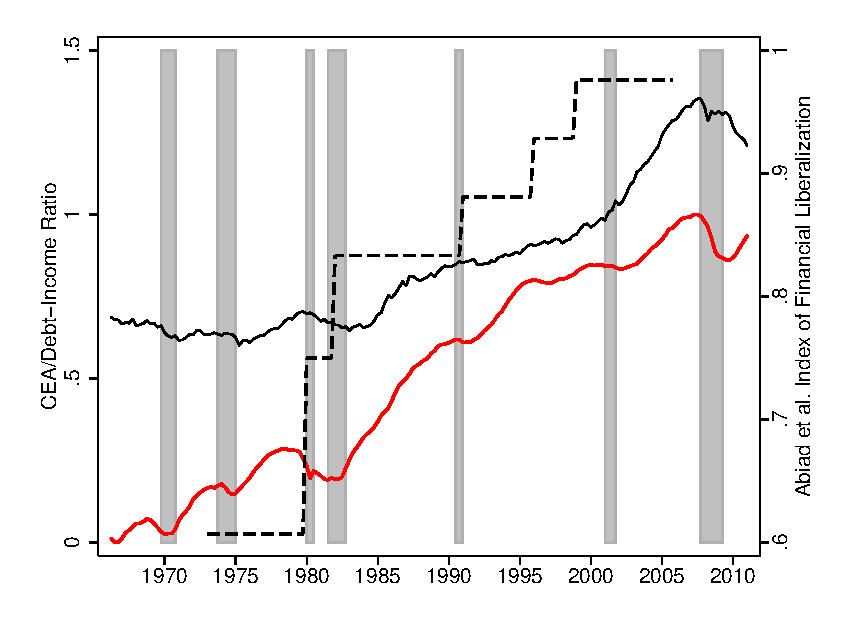
\includegraphics{\econtexRoot/Figures/fCreditAvailability_compare}
%\end{center}
\footnotesize
Legend: Debt--disposable income ratio: Thin black line, CEA index: Thick red/grey line, the \cite{abiadEtAl_FinReforms} Index of Financial Liberalization: Dashed black line. Shading---NBER recessions.\\[0mm]
\tiny Sources: Federal Reserve, accumulated scores from the question on change in the banks' willingness to provide consumer installment loans from the Senior Loan Officer Opinion Survey on Bank Lending Practices, \url{http://www.federalreserve.gov/boarddocs/snloansurvey/}; \cite{abiadEtAl_FinReforms}; Flow of Funds, Board of Governors of the Federal Reserve System.
\end{figure}


Figure~\ref{fCreditAvailability} compares three measures of credit availability: our baseline CEA index, the Index of Financial Liberalization constructed by \cite{abiadEtAl_FinReforms} for a number of countries including the United States, and the ratio of household liabilities to disposable income.

The \citeauthor{abiadEtAl_FinReforms} index is a mixture of indicators of financial development: credit controls and reserve requirements, aggregate credit ceilings, interest rate liberalization, banking sector entry, capital account transactions, development of securities markets and banking sector supervision. The correlation coefficient between this measure and CEA is about 90 percent.

For comparison, the figure also includes the ratio of liabilities to disposable income (from the Flow of Funds), which is however determined influenced by the interaction between credit supply and demand.




\section*{Appendix 2: Stochastic Properties of Aggregate Disposable Income}

\subsection*{Measurement of Disposable Income}

\begin{figure}
\caption{Growth of Real Disposable Income (Percent) \label{fDispIncG}}
%\begin{center}
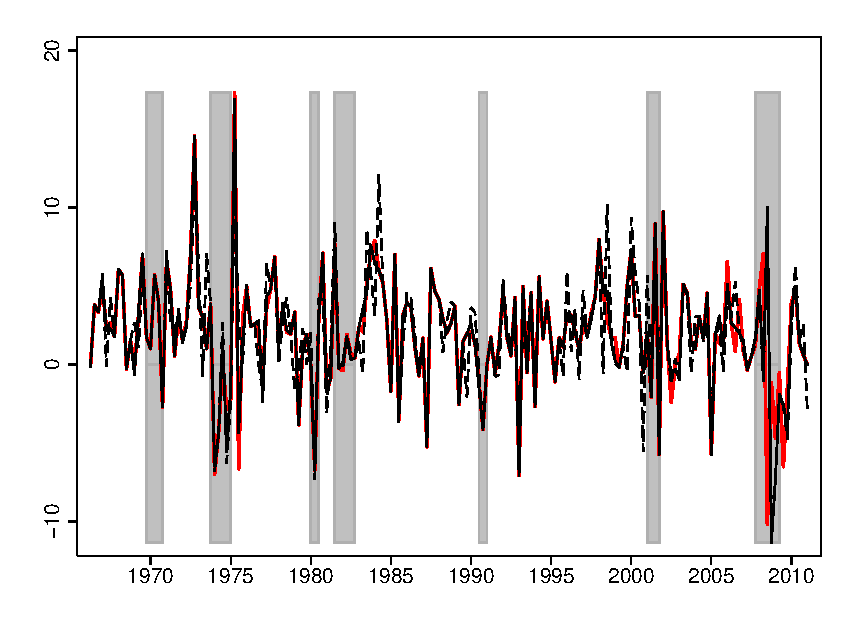
\includegraphics{\econtexRoot/Figures/fDispIncG}
\footnotesize
Legend: BEA disposable income: Thick red/grey line,  ``Less cleaned'' disposable income series: Thin black line, ``More cleaned'' disposable income series: Dashed black line. Shading---NBER recessions.\\[0mm]
\tiny Sources: Bureau of Economic Analysis, authors' calculations.
\end{figure}

\begin{figure}
\caption{Personal Saving Rate (Percent of Disposable Income) \label{fPSRcompare}}
%\begin{center}
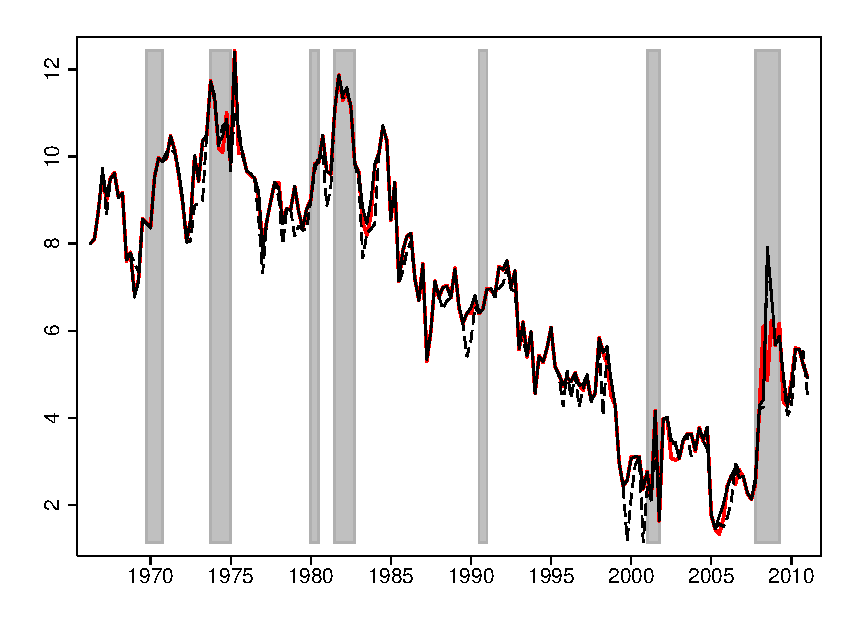
\includegraphics{\econtexRoot/Figures/fPSRcompare}
%\end{center}
\footnotesize
Legend: BEA personal saving rate: Thick red/grey line, PSR calculated with the ``less cleaned'' income series: Thin black line, PSR calculated with the ``more cleaned'' income series: Dashed black line. Shading---NBER recessions.\\[0mm]
\tiny Sources: Bureau of Economic Analysis, authors' calculations.
\end{figure}

This appendix investigates the properties of three measures of disposable income: the official series produced by the BEA and two alternative ``cleaned'' series, in which we aim to exclude transitory income shocks due to temporary events, such as weather and fiscal policy. Specifically, we have removed the following events from the official disposable income series using regressions:
\bi
\item The dollar amounts of temporary rebate checks during 1975, 2008, and 2009 fiscal stimulus episodes.
\item Dummies for the 20 costliest tropical cyclones using data from the National Weather Service.
\item Dummies for quarters with unusually high or low cooling degree days, and unusually high or low heating degree days (the dummy has a value of 1 whenever the seasonally-adjusted series are more than 2 standard deviations above or below its mean).
\item Dummies for quarters with unusually high or low national temperature, and unusually high or low precipitation (again, using the 2 standard deviations criterion).
\item Separate dummies for snowstorms or heat waves which were deemed unusually extensive and damaging (these events do not necessarily overlap with the episodes identified from the national temperature and cooling/heating degree days data).
\ei

The ``less cleaned'' disposable income series removes from published data the contributions of stimulus and heating/cooling day extremes. The ``more cleaned'' series removes all the sources of transitory fluctuations outlined above.



\subsection*{Stochastic Properties of Disposable Income and Saving for a Rainy Day}

The classic paper by \cite{cam87} derived that the permanent income hypothesis implies that saving is negatively  related to future expected income growth.  This appendix investigates the univariate stochastic properties of disposable income and the relationship between saving and income, or the lack of it, in Tables~\ref{tUnivarYPSR} and \ref{tCampbell87}, respectively.

Table~\ref{tUnivarYPSR} documents that all three disposable income series are statistically indistinguishable from a random walk. This means that (changes in) the series are unpredictable using their own lags. In particular, for the income series in log-level, the first autocorrelations are very close to 1 and the augmented Dickey--Fuller test does not reject the null of a unit root. In contrast, for income \emph{growth}, the first and other autocorrelations are zero, as also documented by the p values of the Box--Ljung Q statistic, and the ADF test (of course) strongly rejects  a unit root.

Table~\ref{tCampbell87} reports the estimates of $\alpha_1$ the sensitivity of the saving rate to future income growth:
\be
s_t=\alpha_0+\alpha_1 \Delta y_{t+1}+ \varepsilon_t, \label{cambellRainyDayReg}
\ee
which is motivated by \cite{cam87}, who derives that under the permanent income hypothesis the coefficient $\alpha_1$ is negative, as households save more when they are pessimistic about future income growth.

Overall, the estimates suggest that coefficient $\alpha_1$ is statistically insignificant and small, especially when the full sample, 1966q2--2011q1, is used and when income growth $\Delta y_{t+2}$ enters the regression \eqref{cambellRainyDayReg}, which might be justified because of time aggregation issues. While there is some evidence of a negative coefficient in the pre-1985 sample (which overlaps with the sample 1953q2--1984q4 considered by \cite{cam87}), the relationship seems to break down in the past 20 years.

\input ./LaTeX/AppendixSeveranceBody.tex

\newpage

\input./Tables/tOLS_prelim_time.tex
\input./Tables/tOLS02.tex
\input./Tables/tOLS_subSample.tex
\input./Tables/tPred.tex
\input./Tables/tStructEst.tex
\input./Tables/tOLS_prelim_time_model.tex
\input./Tables/tUnivarYPSR.tex
\input./Tables/tCampbell87.tex

\end{document}
